% !TEX root = q3_section.tex
% 问题三可直接粘贴进 Overleaf 的模型章。
% 所有未签收数字使用宏；不得把宏展开成文档复核数字。
% 编译本文件需 cumcmthesis 或 article + ctex。Overleaf 主稿请 % !TEX root = q3_section.tex
% 问题三可直接粘贴进 Overleaf 的模型章。
% 所有未签收数字使用宏；不得把宏展开成文档复核数字。
% 编译本文件需 cumcmthesis 或 article + ctex。Overleaf 主稿请 % !TEX root = q3_section.tex
% 问题三可直接粘贴进 Overleaf 的模型章。
% 所有未签收数字使用宏；不得把宏展开成文档复核数字。
% 编译本文件需 cumcmthesis 或 article + ctex。Overleaf 主稿请 % !TEX root = q3_section.tex
% 问题三可直接粘贴进 Overleaf 的模型章。
% 所有未签收数字使用宏；不得把宏展开成文档复核数字。
% 编译本文件需 cumcmthesis 或 article + ctex。Overleaf 主稿请 \input{q3_section}。

% ---------- 未核数字宏（队长写入 results_summary.md 后再替换）----------
\newcommand{\QThreeUnsigned}{[待签收]}
\newcommand{\QThreeMainCost}{\QThreeUnsigned}
\newcommand{\QThreeMZeroCost}{\QThreeUnsigned}
\newcommand{\QThreeSaveVsMZero}{\QThreeUnsigned}
\newcommand{\QThreeSavePct}{\QThreeUnsigned}
\newcommand{\QThreeEmergDrop}{\QThreeUnsigned}
\newcommand{\QThreeSettleLift}{\QThreeUnsigned}
\newcommand{\QThreeYearEndA}{1200}
\newcommand{\QThreeYearEndB}{6000}

% ============================================================
\subsection{问题三：预测更新下的购电调整与储能滚动调度}
% ============================================================

\subsubsection{问题的数学本质与同问题二的衔接}

问题三并不改写问题一、问题二已经成立的公共母线能量平衡、储能效率和跨日 SOC 传递，真正新增的困难是\textbf{信息到达方式}：每日 0:00、6:00、12:00、18:00 各得到一条未来 24 小时光伏点预测，题目允许据此调整尚未执行的购电策略，并且上调、下调分别按交易时刻电价的 1.5 倍与 50\% 结算。因此本问的对象不再是“一次性锁定的日前额度”，而是一条随预测更新而可能改写的承诺过程
\[
g^{0}_{d,\cdot}\;\longrightarrow\;
g^{\tau}_{d,\cdot}\ (\tau\in\{6{:}00,12{:}00,18{:}00\})\;\longrightarrow\;
g^{F}_{d,\cdot},
\]
其中 \(g^{F}\) 是该时段到来前最后一次有效承诺。

若把问题二的“全日锁定、日内只靠储能和紧急购电补救”原样搬来，将直接放弃题目明确给出的三次更新权利，必然高估紧急购电。反之，若在 6:00 之后仍允许改写 0:00--6:00 已经执行的电量，或把尚未发布的附件 3 预测、当天未来实际光伏当作当前决策输入，则模型在信息上优于任何可执行策略。由于问题二已经把普通购电承诺与实时物理补救分开，问题三只需在同一框架上打开放宽条件：\textbf{承诺层允许按更新时点改写未执行时段，执行层仍然只能使用已观测状态}。储能与紧急购电继续承担补救角色，不能替代本可在最近一次更新点完成的正常购电调整。

本问与问题二的衔接建立在最新政策一致设计之上：日前层只在单一因果基准预测轨迹上求线性规划，\(K=8\) 仅用于风险储备与日内残差匹配，不再给每条历史情景单独优化储能；日内仍是锁定普通购电后的滚动执行。问题三保留同一套公共母线物理与跨日 SOC，只把“全日锁定”放宽为 6:00、12:00、18:00 可改未执行承诺。已签收附件 \texttt{result2.xlsx} 目前仍是原 \(K=8\) 情景规划口径；政策一致路径是否替换该正式文件由队长决定，\textbf{不改变}本节的结算、更新窗口和滚动 LP。

负荷预测方面，问题三固定采用透明基线 \(m_1\)：最近至多 4 个同星期历史日逐时段均值，记为 \(\widehat L_{d,t}\)。政策一致全年部署路径在 2--12 月有 207/334 日选用 \(m_3\)、56 日选用 \(m_2\)，仅 71 日为 \(m_1\)，因此二者只是结构同类，\textbf{不是同一预测器}；问题三也不随问题二每 14 日在线切换。48 小时终端价值与新问题二一致，由次日基准预测 LP 的支持割近似，数值必须按附件 3 的更新口径重新估计，不得搬用问题二的切面，也不得再写成旧方案的“全路径情景储能补救”。

\subsubsection{符号、信息集与调整结算}

一天划分为 \(T=144\) 个 10 分钟时段，\(\Delta t=1/6\) h。附件 2 的功率先化为时段能量 \(L_{d,t}=\ell_{d,t}\Delta t\)、\(P_{d,t}=\rho_{d,t}\Delta t\)。更新时点集合为 \(\mathcal U=\{0{:}00,6{:}00,12{:}00,18{:}00\}\)。令 \(\mathcal T_\tau\) 为 \(\tau\) 之后当日尚未执行的时段；6:00、12:00、18:00 的首个可改时段分别为 6:10、12:10、18:10。

\begin{table}[H]
\centering
\caption{问题三新增或含义发生变化的主要符号}
\label{tab:q3-symbols}
\small
\begin{tabular}{cll}
\toprule
符号 & 含义 & 单位 / 边界 \\
\midrule
\(g^{0}_{d,t}\) & 当日 0:00 制订的普通购电原计划 & kWh，\(g^{0}\ge 0\) \\
\(g_{d,t}\) & 当前版本承诺；时段到来前的最终值为 \(g^{F}_{d,t}\) & kWh，\(g\ge 0\) \\
\(x_{d,t}\) & 从当期承诺中实际取用的普通电量 & \(0\le x\le g^{F}\) \\
\(e_{d,t}\) & 实时紧急购电 & kWh，\(e\ge 0\) \\
\(\phi_t(g^{0},g^{F})\) & 相对 0:00 原计划的计划--调整结算 & 元 \\
\(\widehat P^{\tau}_{d,t}\) & 时点 \(\tau\) 发布后映射得到的 10 分钟光伏预测 & kWh \\
\(\widehat L_{d,t}\) & 日初因果负荷预测（执行前缀外保持不变） & kWh \\
\(VoI_{\tau}\) & 时点 \(\tau\) 上“允许调整”相对“维持承诺”的预测成本差 & 元 \\
\(V_{d+1}(E_{d,144})\) & 下一日 SOC 的虚拟到达成本，不计入当日账单 & 元 \\
\bottomrule
\end{tabular}
\end{table}

充放电 \(c_{d,t},r_{d,t}\)、弃光 \(w_{d,t}\) 与 SOC \(E_{d,t}\) 沿用问题一的公共母线口径：功率上限 \(5000\Delta t\) kWh，SOC 窗口 \([1200,10800]\) kWh，\(\eta_c=\eta_d=\sqrt{0.9}\)，\(E_{2025\text{-}01\text{-}01,0}=6000\) kWh，且 \(E_{d+1,0}=E_{d,144}\)。已签收问题二与政策一致全年部署路径均在 2025-12-31 日末落到 \(1200\) kWh，故主核算取年末 \(E_{\mathrm{end}}=\QThreeYearEndA\) kWh，作为与问题二可比的统一库存边界；\(\QThreeYearEndB\) kWh 仅作库存中性敏感性。该选择不是题面规定，也不是社区运行规律。2 月初库存两条问题二路径并不相同（已签收约 \(2645\) kWh，政策一致部署约 \(1228\) kWh），问题三必须从 1 月 1 日 \(6000\) kWh 沿自身决策传递 SOC，不得借用问题二的 2 月 1 日状态。

\paragraph{主结算口径。}
题目同时出现“原计划高于调整量按 50\% 结算、调整量高于原计划按 1.5 倍结算”。若把“原计划的正常电费”与“下调违约费”对取消量同时全额累加，取消部分会被收一次正常价再收一次 50\% 价。经济上可执行、且不重复计价的读法是：最终实际采购的 \(g^{F}\) 按正常价结算，相对 \(g^{0}\) 的偏差按半价的绝对值附加。于是
\begin{equation}
\label{eq:q3-phi}
\phi_t(g^{0},g^{F})=p_t g^{F}+\frac12 p_t\lvert g^{F}-g^{0}\rvert
=
\begin{cases}
p_t g^{F}+\dfrac12 p_t(g^{0}-g^{F}), & g^{F}\le g^{0},\\[4pt]
p_t g^{0}+\dfrac32 p_t(g^{F}-g^{0}), & g^{F}>g^{0}.
\end{cases}
\end{equation}
同一时段可能在 6:00、12:00、18:00 被多次讨论，但账单始终锚定该日 0:00 的 \(g^{0}\)，不对未执行的中间版本逐笔叠加。式~\eqref{eq:q3-phi} 是本文对题意的主解释，不是市场规则的唯一数学定理；相邻版本逐次结算只进入附录敏感性，不进入主结论。

目标是最小化实际发生的购电成本
\begin{equation}
\label{eq:q3-total-cost}
\min C=\sum_{d,t}\Bigl[\phi_t\bigl(g^{0}_{d,t},g^{F}_{d,t}\bigr)+5p_t e_{d,t}\Bigr],
\end{equation}
而不是最小化某一次计划量。\(V_{d+1}\) 只出现在滚动优化的目标中，用于避免有限视域末端把电池不合理地耗尽，不计入~\eqref{eq:q3-total-cost}。

\paragraph{因果预测。}
附件 3 给出逐小时光伏点预测。每次更新以\textbf{该时点刚观测到的实际光伏}为锚点，再与随后 24 个整点预报线性插值到 10 分钟网格，得到 \(\widehat P^{\tau}\)。不得使用未来附件 2 实际光伏做插值节点。负荷没有单独预报附件：主模型对计划日 \(d\) 取
\begin{equation}
\label{eq:q3-load}
\widehat L_{d,t}=\frac1{|\mathcal H_d|}\sum_{j\in\mathcal H_d}L_{j,t},
\end{equation}
其中 \(\mathcal H_d\) 是日期严格早于 \(d\) 的最近至多 4 个同星期历史日。6:00/12:00/18:00 规划未来时段时仍使用该日 0:00 已形成的 \(\widehat L\)，不读取当天尚未发生的附件 2 负荷。每 10 分钟执行当前一步时，才以当期真实 \((L_{d,t},P_{d,t})\) 闭合能量平衡。附件 2 当日完整负荷曲线仅作为理想化对照 \(\texttt{actual\_load\_proxy}\)，用于量化“若负荷被完美预知”的信息价值，不得作为主方案或可执行策略。

图~\ref{fig:q3-info} 给出承诺锁定窗口与信息集；图~\ref{fig:q3-phi} 给出主结算与重复计费读法的对比。

\begin{figure}[H]
\centering
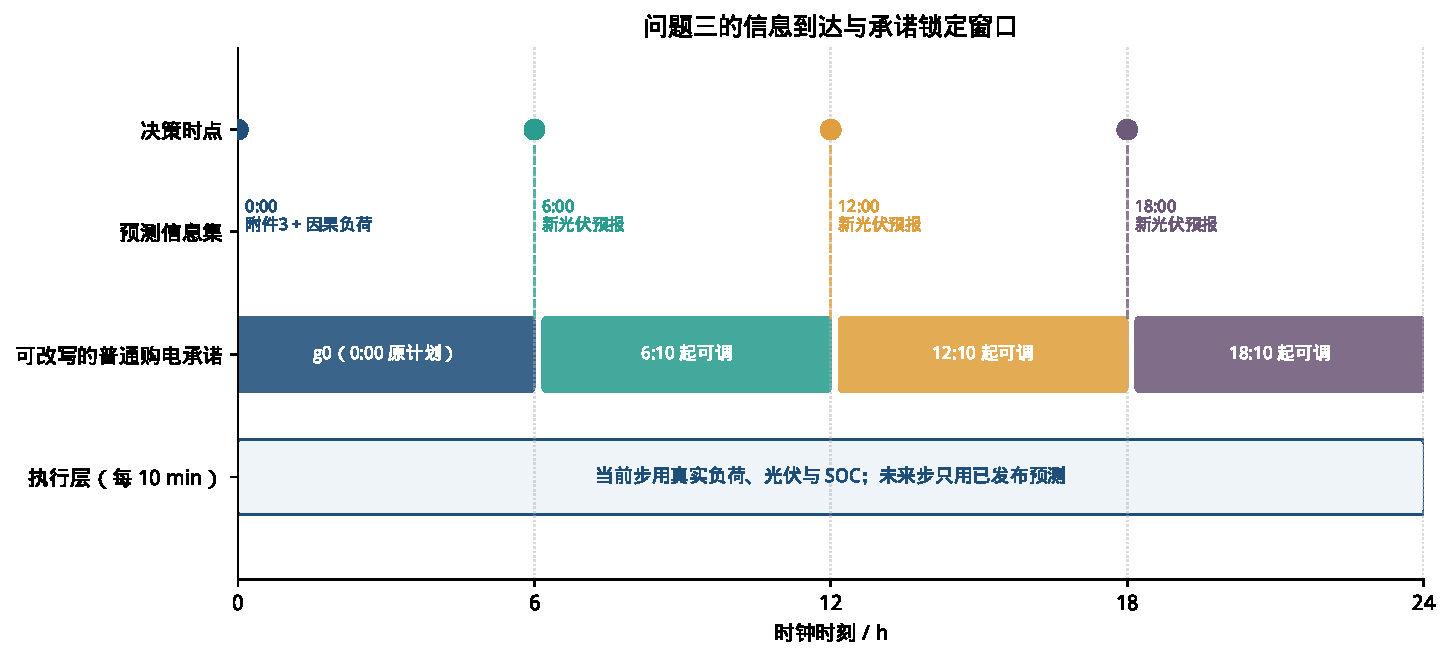
\includegraphics[width=0.95\textwidth]{../fig/q3_paper/fig3_info_timeline.pdf}
\caption{问题三的信息到达与承诺改写窗口。虚线为预测发布时间；色块表示该时点之后尚未执行、因而可以改写的普通购电承诺。执行层始终只在当前 10 分钟使用真实负荷与光伏。}
\label{fig:q3-info}
\end{figure}

\begin{figure}[H]
\centering
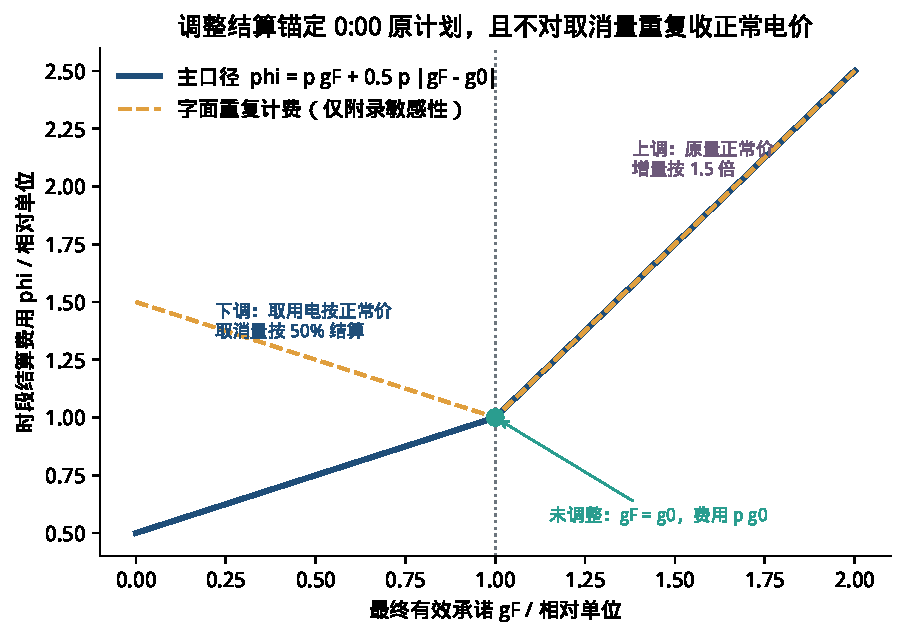
\includegraphics[width=0.72\textwidth]{../fig/q3_paper/fig3_settlement_phi.pdf}
\caption{以 0:00 原计划为锚点的调整结算。实线为主口径~\eqref{eq:q3-phi}；虚线把下调取消量同时按正常价和 50\% 计价，只作附录敏感性，以免把题意歧义写成唯一市场事实。}
\label{fig:q3-phi}
\end{figure}

\subsubsection{主模型：四时点滚动重优化}

物理可行性与问题一、问题二相同。公共母线能量平衡与 SOC 转移为
\begin{equation}
\label{eq:q3-balance}
x_{d,t}+e_{d,t}+P_{d,t}-w_{d,t}+r_{d,t}=L_{d,t}+c_{d,t},
\end{equation}
\begin{equation}
\label{eq:q3-soc}
E_{d,t}=E_{d,t-1}+\eta_c c_{d,t}-\frac{r_{d,t}}{\eta_d}.
\end{equation}
普通购电只能在当期承诺内取用，\(0\le x_{d,t}\le g_{d,t}\)；多余承诺已经按~\eqref{eq:q3-phi} 结算，但不能凭空转移到其他时段。跨时搬运只能经过“购电或光伏 \(\to\) 充电 \(\to\) SOC \(\to\) 放电”。在正电价、无上网收益且电池有损耗时，同时充放电被更低损耗的等价解支配；求解后仍审计 \(c_{d,t}r_{d,t}=0\)。

\paragraph{M0：0:00 后不调整。}
以 0:00 的 \((\widehat L,\widehat P^{0})\) 制订 \(g^{0}\)，此后强制 \(g^{F}=g^{0}\)。它回答“新预测总体上有没有货币价值”：任何允许更新的策略，必须在同一初始 SOC、同一结算和同一执行规则下给出更低的实现成本~\eqref{eq:q3-total-cost}，否则更新权利只是名义上的。

\paragraph{M1：每次更新都评估并求解。}
设更新时刻 \(\tau\) 的当前真实 SOC 为 \(E_{d,\tau}\)，更新前承诺为 \(g^{\mathrm{pre}}\)。在剩余时域 \(\mathcal T_\tau\) 上解
\begin{equation}
\label{eq:q3-m1}
\boxed{
\left\{
\begin{aligned}
\min_{g,x,e,c,r,w,E}\quad
&\sum_{t\in\mathcal T_\tau}
\bigl[\phi_t(g^{0}_{d,t},g_{d,t})+5p_t e_{d,t}\bigr]
+V_{d+1}(E_{d,144}),\\
&g_{d,t}=g^{\mathrm{pre}}_{d,t},\qquad t\notin\mathcal T_\tau,\\
&0\le x_{d,t}\le g_{d,t},\qquad g_{d,t}\ge 0,\\
&\text{以及~\eqref{eq:q3-balance}--\eqref{eq:q3-soc} 与功率、SOC、弃光边界。}
\end{aligned}
\right.}
\end{equation}
规划阶段的平衡使用 \((\widehat L_{d,t},\widehat P^{\tau}_{d,t})\)；执行当前一步时改用真实 \((L_{d,t},P_{d,t})\)，只实施本步动作，下一时段带入真实 SOC 再滚动。这不是预知未来光伏或未来负荷的事后最优。因为 \(g=g^{\mathrm{pre}}\) 始终可行，并且调整价格已经进入目标，模型只有在改计划后仍能降低预计总成本时才会离开原承诺。因而 M1 的“每次更新”是指每次都求解，而不是强迫计划变化。

\paragraph{M6：用信息价值记录是否实施调整。}
在 \(\tau\in\{6{:}00,12{:}00,18{:}00\}\) 计算
\begin{equation}
\label{eq:q3-voi}
\begin{aligned}
J^{\mathrm{fix}}_{\tau}&=\min\{J_{\tau}:g_{d,t}=g^{\mathrm{pre}}_{d,t},\ t\in\mathcal T_\tau\},\\
J^{\mathrm{free}}_{\tau}&=\min\{J_{\tau}:g_{d,t}\ge 0,\ t\in\mathcal T_\tau\},\\
VoI_{\tau}&=J^{\mathrm{fix}}_{\tau}-J^{\mathrm{free}}_{\tau}.
\end{aligned}
\end{equation}
仅当 \(VoI_{\tau}>\varepsilon\) 时写入新承诺，否则维持 \(g^{\mathrm{pre}}\)。\(\varepsilon=0.01\) 元取求解器货币容差，只防止无意义的浮点微调。当保持原承诺可行、调整费进入目标且 \(\varepsilon\to 0\) 时，M1 与 M6 给出同一经济最优解。因此 M6 不是第二个独立主算法，而是 M1 的可解释实施层：它把“新预测值不值得用”写成逐时点的 \(VoI\) 台账。真正有信息含义的比较是
\[
\text{M0},\quad
\text{M1/M6},\quad
M_{6},\ M_{12},\ M_{18},
\]
其中后三个消融各自只开放一个更新时点，用于回答哪一次预报对实现成本最关键。图~\ref{fig:q3-voi} 给出该实施逻辑。

\begin{figure}[H]
\centering
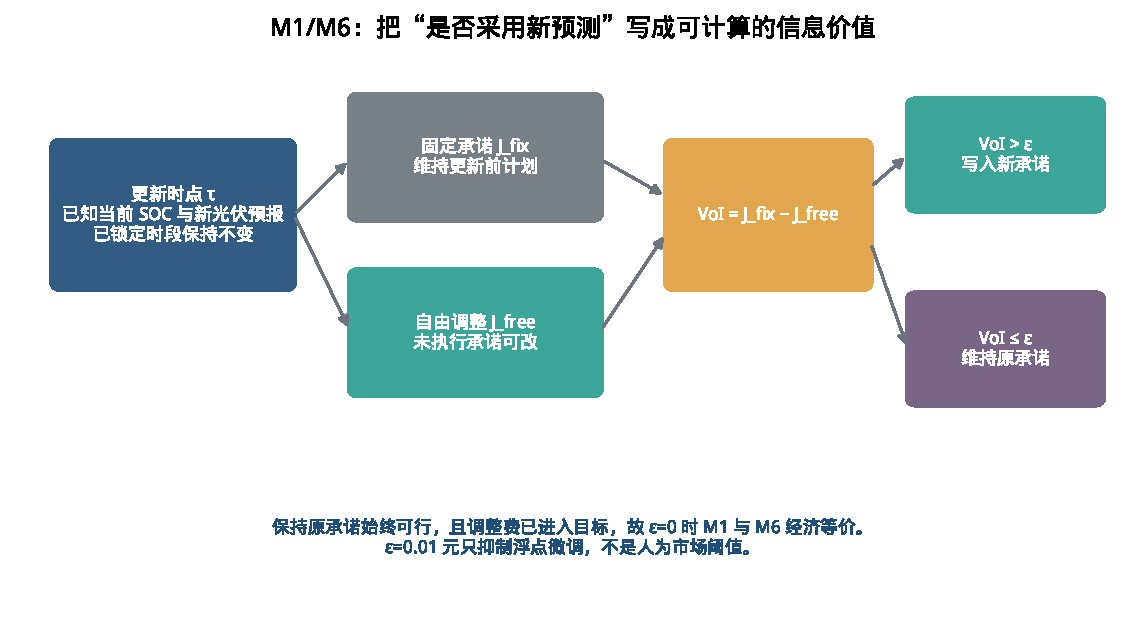
\includegraphics[width=0.92\textwidth]{../fig/q3_paper/fig3_voi_decision.pdf}
\caption{更新时点上的信息价值判定。由于不调整始终可行，\(VoI\) 不会人为制造成本差；单时点消融而不是 M1 对 M6 的成本差，才是“哪个时刻的预测值得使用”的证据。}
\label{fig:q3-voi}
\end{figure}

\paragraph{终端价值。}
日末不强制回到日初 SOC。为避免最后数小时透支电池，优化视域延长到次日，或等价加入到达项 \(V_{d+1}(E_{d,144})\)。该项与问题二政策一致方案相同：由次日基准预测 LP（而非情景全路径补救）在若干 SOC 样本上生成凸支持割，并以弦线--切面间隙作为误差证书。预测输入改用问题三的因果负荷与附件 3 更新口径。它只引导今日末库存，次日购电计划必须到次日 0:00 重新制订，不得提前写入结果文件或重复计费。

\subsubsection{求解算法}

式~\eqref{eq:q3-m1} 在固定预测轨迹下是线性规划：\(\phi_t\) 的绝对值由非负上、下调变量线性化，能量平衡与 SOC 均为线性等式，容量与功率均为盒约束。主求解使用 LP（HiGHS）；若出现数值上的同时充放电，先以最小吞吐量作词典序次目标，仅在仍不能消除时用互斥二元变量复核。选择 LP 而不是遗传算法或完整多阶段随机动态规划，是因为：题目的调整费和紧急电价已经给出可加的货币目标；承诺跨时段的耦合由 SOC 线性传递；计算瓶颈在于全年、多策略、每 10 分钟滚动，而不是非凸组合爆炸。完整情景树（规格中的 M5）能够刻画未发生光伏误差的条件残差，但要求购电承诺跨情景一致、控制动作服从信息历史，不能把每条未来轨迹的储能当作日初指令。M5 只作为不确定性扩展，不替代 M1/M6 的主结果；在其全年审计完成前，正文不把问题三称为严格多阶段随机最优控制。

算法流程如下。对每个策略、每一日：用~\eqref{eq:q3-load} 与 0:00 光伏映射形成日初信息并求解 \(g^{0}\)；在允许的更新点比较 \(J^{\mathrm{fix}}\) 与 \(J^{\mathrm{free}}\)；每个 10 分钟只执行当前动作并更新真实 SOC；日成本按~\eqref{eq:q3-total-cost} 归集。全年比较时，每个策略必须从 2025-01-01 的 6000 kWh 起沿\textbf{自身}决策连续传递 SOC，不得借用 M0 或其他策略的库存路径。1 月用于状态预热与预测历史，题设结果表覆盖 2--12 月；若报告年度成本，须写明是 1--12 月完整核算还是 2--12 月输出区间，二者不得混报。

\subsubsection{结果与机制解释}
\label{sec:q3-results}

本节数字一律待队长把因果负荷主路径写入 \texttt{results\_summary.md} 后再填。当前两日试算使用了当天完整真实负荷，只证明结算公式、锁定窗口和物理残差链路可运行，不能代表现实可执行的日前/日内策略。

待填的主比较应同时给出总成本、普通结算成本、紧急购电成本和弃光，避免把“调整次数多”直接写成“更好”。预期的机制解释（有签收数字后按实际符号改写，不得预先断言全年排序）是：允许更新的策略如果优于 M0，其来源应是\textbf{减少 5 倍紧急补购}，而普通结算成本完全可能上升——因为上调按 1.5 倍付费，模型只有在避免紧急购电的收益超过调整费时才会增加 \(g\)。单时点消融若出现“仅 6:00 更新的实现成本劣于 M0”，原因通常是过早下调后，后续真实光伏/负荷偏差无法在已锁定期内用正常购电挽回，只能转化为紧急购电或被动弃光；这恰恰说明 \(VoI\) 是当时信息下的预测收益，不是实现路径上的保证收益。18:00 更新若增量很小，则因为剩余时段短、可改电量少，且日末库存已由 48 小时到达项约束。

\begin{table}[H]
\centering
\caption{问题三主比较（因果负荷、线性锚点映射、0:00 锚定结算；数字待签收）}
\label{tab:q3-strategy}
\begin{tabular}{lcccc}
\toprule
策略 & 总成本 / 元 & 相对 M0 & 普通结算 / 元 & 紧急成本 / 元 \\
\midrule
M0（不调整） & \QThreeMZeroCost & --- & \QThreeUnsigned & \QThreeUnsigned \\
\(M_{6}\) 仅 6:00 & \QThreeUnsigned & \QThreeUnsigned & \QThreeUnsigned & \QThreeUnsigned \\
\(M_{12}\) 仅 12:00 & \QThreeUnsigned & \QThreeUnsigned & \QThreeUnsigned & \QThreeUnsigned \\
\(M_{18}\) 仅 18:00 & \QThreeUnsigned & \QThreeUnsigned & \QThreeUnsigned & \QThreeUnsigned \\
M1/M6（三点均评估） & \QThreeMainCost & \QThreeSavePct & \QThreeSettleLift & \QThreeEmergDrop \\
\bottomrule
\end{tabular}
\end{table}

指定展示日的计划购电量、调整购电量、四小时充放电与紧急购电按题设 \texttt{result3.xlsx} 列出。正文须同时说明该日 0:00 原计划、各更新点 \(VoI\) 以及调整方向，避免只贴最终 \(g^{F}\)。题设导出区间为 2025-02-01 至 2025-12-31；1 月不写入结果表，但跨日 SOC 必须从年初连续而来。

不得把问题二已签收的 2--12 月成本 14{,}456{,}670.55 元，或政策一致部署路径的 2--12 月成本，与问题三年度成本直接相减。两问结算对象不同（问题二按锁定额度 \(q\) 付费，问题三按 \(\phi(g^{0},g^{F})\) 付费），信息集也不同。对照只能在队长同时签收两问主口径、并统一首末 SOC 与核算区间之后，分项列出计划/调整/紧急三项。

\subsubsection{验证、敏感性与表述边界}

必须通过、且论文只声称“通过数值审计”的项目包括：逐 10 分钟能量平衡与 SOC 递推残差达到数值求解量级；SOC、功率、弃光边界无违例；更新点之前的 \(g\) 不被改写；\(x\le g\)；无同时充放电；\(\phi\) 对上调、下调、未调三类样本与分段定义一致；主模型对当天尚未发生的负荷做扰动时，当时计划不变。\(\texttt{actual\_load\_proxy}\) 必须单独成表，不能并入主比较。

小时预报到 10 分钟的线性锚点映射不是附件唯一规定，分段常数映射只作敏感性。主结算不是题意的唯一读法，相邻版本逐次结算只作附录。在这些全年组合跑完以前，只可以写“两日回归样本未改变审计结论”，不可以写“全年映射与结算解释下策略排序均稳健”。年末 1200 kWh 与 6000 kWh 是核算边界：前者允许释放期初库存，后者要求年末仍保留该库存；成本差应首先解释为库存会计，其次才检查是否改变策略排序。控制器能够即时获得当前负荷/光伏，是本文的控制信息假设，题目未给出通信延迟，故不把结果写成工程部署方案。

图~\ref{fig:q3-overview} 总结问题三在四问主线中的位置：它只放宽承诺改写的时点，不另起一套储能物理。

\begin{figure}[H]
\centering
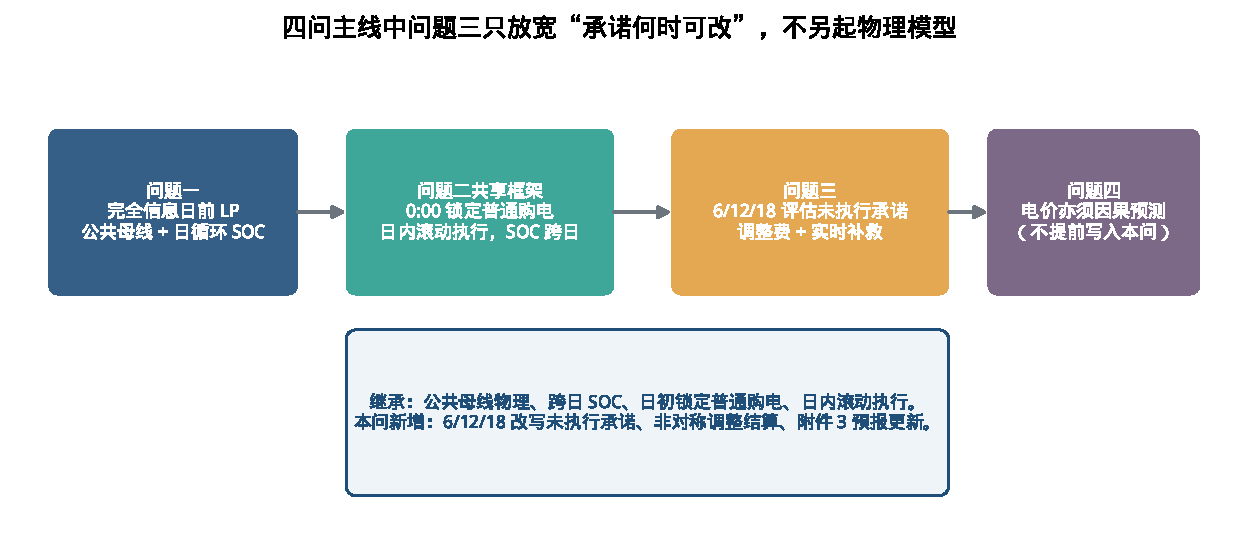
\includegraphics[width=0.96\textwidth]{../fig/q3_paper/fig3_q2_to_q3_overview.pdf}
\caption{问题三在全文主线中的位置。评委从本图应读出：储能物理连续继承，信息集按问递进；本问只放宽普通购电承诺的改写时点，并把调整费计入目标。}
\label{fig:q3-overview}
\end{figure}

% 摘要可用段落（数字仍为宏）
% \textbf{针对问题三，}由于光伏预测在 0:00、6:00、12:00、18:00 更新，若继续全日锁定普通购电，将放弃题目允许的调整权并放大紧急购电。因此以 0:00 原计划为唯一结算锚点，建立计入非对称调整费的剩余时域滚动 LP，并用预测成本差 \(VoI\) 记录是否实施调整。主方案在因果负荷与线性锚点映射下的实现成本为 \QThreeMainCost 元，相对从不调整的 M0 为 \QThreeSavePct。该差额来自紧急购电下降与普通结算变化的对冲，而不是取消调整费或预知未来实际曲线。
。

% ---------- 未核数字宏（队长写入 results_summary.md 后再替换）----------
\newcommand{\QThreeUnsigned}{[待签收]}
\newcommand{\QThreeMainCost}{\QThreeUnsigned}
\newcommand{\QThreeMZeroCost}{\QThreeUnsigned}
\newcommand{\QThreeSaveVsMZero}{\QThreeUnsigned}
\newcommand{\QThreeSavePct}{\QThreeUnsigned}
\newcommand{\QThreeEmergDrop}{\QThreeUnsigned}
\newcommand{\QThreeSettleLift}{\QThreeUnsigned}
\newcommand{\QThreeYearEndA}{1200}
\newcommand{\QThreeYearEndB}{6000}

% ============================================================
\subsection{问题三：预测更新下的购电调整与储能滚动调度}
% ============================================================

\subsubsection{问题的数学本质与同问题二的衔接}

问题三并不改写问题一、问题二已经成立的公共母线能量平衡、储能效率和跨日 SOC 传递，真正新增的困难是\textbf{信息到达方式}：每日 0:00、6:00、12:00、18:00 各得到一条未来 24 小时光伏点预测，题目允许据此调整尚未执行的购电策略，并且上调、下调分别按交易时刻电价的 1.5 倍与 50\% 结算。因此本问的对象不再是“一次性锁定的日前额度”，而是一条随预测更新而可能改写的承诺过程
\[
g^{0}_{d,\cdot}\;\longrightarrow\;
g^{\tau}_{d,\cdot}\ (\tau\in\{6{:}00,12{:}00,18{:}00\})\;\longrightarrow\;
g^{F}_{d,\cdot},
\]
其中 \(g^{F}\) 是该时段到来前最后一次有效承诺。

若把问题二的“全日锁定、日内只靠储能和紧急购电补救”原样搬来，将直接放弃题目明确给出的三次更新权利，必然高估紧急购电。反之，若在 6:00 之后仍允许改写 0:00--6:00 已经执行的电量，或把尚未发布的附件 3 预测、当天未来实际光伏当作当前决策输入，则模型在信息上优于任何可执行策略。由于问题二已经把普通购电承诺与实时物理补救分开，问题三只需在同一框架上打开放宽条件：\textbf{承诺层允许按更新时点改写未执行时段，执行层仍然只能使用已观测状态}。储能与紧急购电继续承担补救角色，不能替代本可在最近一次更新点完成的正常购电调整。

本问与问题二的衔接建立在最新政策一致设计之上：日前层只在单一因果基准预测轨迹上求线性规划，\(K=8\) 仅用于风险储备与日内残差匹配，不再给每条历史情景单独优化储能；日内仍是锁定普通购电后的滚动执行。问题三保留同一套公共母线物理与跨日 SOC，只把“全日锁定”放宽为 6:00、12:00、18:00 可改未执行承诺。已签收附件 \texttt{result2.xlsx} 目前仍是原 \(K=8\) 情景规划口径；政策一致路径是否替换该正式文件由队长决定，\textbf{不改变}本节的结算、更新窗口和滚动 LP。

负荷预测方面，问题三固定采用透明基线 \(m_1\)：最近至多 4 个同星期历史日逐时段均值，记为 \(\widehat L_{d,t}\)。政策一致全年部署路径在 2--12 月有 207/334 日选用 \(m_3\)、56 日选用 \(m_2\)，仅 71 日为 \(m_1\)，因此二者只是结构同类，\textbf{不是同一预测器}；问题三也不随问题二每 14 日在线切换。48 小时终端价值与新问题二一致，由次日基准预测 LP 的支持割近似，数值必须按附件 3 的更新口径重新估计，不得搬用问题二的切面，也不得再写成旧方案的“全路径情景储能补救”。

\subsubsection{符号、信息集与调整结算}

一天划分为 \(T=144\) 个 10 分钟时段，\(\Delta t=1/6\) h。附件 2 的功率先化为时段能量 \(L_{d,t}=\ell_{d,t}\Delta t\)、\(P_{d,t}=\rho_{d,t}\Delta t\)。更新时点集合为 \(\mathcal U=\{0{:}00,6{:}00,12{:}00,18{:}00\}\)。令 \(\mathcal T_\tau\) 为 \(\tau\) 之后当日尚未执行的时段；6:00、12:00、18:00 的首个可改时段分别为 6:10、12:10、18:10。

\begin{table}[H]
\centering
\caption{问题三新增或含义发生变化的主要符号}
\label{tab:q3-symbols}
\small
\begin{tabular}{cll}
\toprule
符号 & 含义 & 单位 / 边界 \\
\midrule
\(g^{0}_{d,t}\) & 当日 0:00 制订的普通购电原计划 & kWh，\(g^{0}\ge 0\) \\
\(g_{d,t}\) & 当前版本承诺；时段到来前的最终值为 \(g^{F}_{d,t}\) & kWh，\(g\ge 0\) \\
\(x_{d,t}\) & 从当期承诺中实际取用的普通电量 & \(0\le x\le g^{F}\) \\
\(e_{d,t}\) & 实时紧急购电 & kWh，\(e\ge 0\) \\
\(\phi_t(g^{0},g^{F})\) & 相对 0:00 原计划的计划--调整结算 & 元 \\
\(\widehat P^{\tau}_{d,t}\) & 时点 \(\tau\) 发布后映射得到的 10 分钟光伏预测 & kWh \\
\(\widehat L_{d,t}\) & 日初因果负荷预测（执行前缀外保持不变） & kWh \\
\(VoI_{\tau}\) & 时点 \(\tau\) 上“允许调整”相对“维持承诺”的预测成本差 & 元 \\
\(V_{d+1}(E_{d,144})\) & 下一日 SOC 的虚拟到达成本，不计入当日账单 & 元 \\
\bottomrule
\end{tabular}
\end{table}

充放电 \(c_{d,t},r_{d,t}\)、弃光 \(w_{d,t}\) 与 SOC \(E_{d,t}\) 沿用问题一的公共母线口径：功率上限 \(5000\Delta t\) kWh，SOC 窗口 \([1200,10800]\) kWh，\(\eta_c=\eta_d=\sqrt{0.9}\)，\(E_{2025\text{-}01\text{-}01,0}=6000\) kWh，且 \(E_{d+1,0}=E_{d,144}\)。已签收问题二与政策一致全年部署路径均在 2025-12-31 日末落到 \(1200\) kWh，故主核算取年末 \(E_{\mathrm{end}}=\QThreeYearEndA\) kWh，作为与问题二可比的统一库存边界；\(\QThreeYearEndB\) kWh 仅作库存中性敏感性。该选择不是题面规定，也不是社区运行规律。2 月初库存两条问题二路径并不相同（已签收约 \(2645\) kWh，政策一致部署约 \(1228\) kWh），问题三必须从 1 月 1 日 \(6000\) kWh 沿自身决策传递 SOC，不得借用问题二的 2 月 1 日状态。

\paragraph{主结算口径。}
题目同时出现“原计划高于调整量按 50\% 结算、调整量高于原计划按 1.5 倍结算”。若把“原计划的正常电费”与“下调违约费”对取消量同时全额累加，取消部分会被收一次正常价再收一次 50\% 价。经济上可执行、且不重复计价的读法是：最终实际采购的 \(g^{F}\) 按正常价结算，相对 \(g^{0}\) 的偏差按半价的绝对值附加。于是
\begin{equation}
\label{eq:q3-phi}
\phi_t(g^{0},g^{F})=p_t g^{F}+\frac12 p_t\lvert g^{F}-g^{0}\rvert
=
\begin{cases}
p_t g^{F}+\dfrac12 p_t(g^{0}-g^{F}), & g^{F}\le g^{0},\\[4pt]
p_t g^{0}+\dfrac32 p_t(g^{F}-g^{0}), & g^{F}>g^{0}.
\end{cases}
\end{equation}
同一时段可能在 6:00、12:00、18:00 被多次讨论，但账单始终锚定该日 0:00 的 \(g^{0}\)，不对未执行的中间版本逐笔叠加。式~\eqref{eq:q3-phi} 是本文对题意的主解释，不是市场规则的唯一数学定理；相邻版本逐次结算只进入附录敏感性，不进入主结论。

目标是最小化实际发生的购电成本
\begin{equation}
\label{eq:q3-total-cost}
\min C=\sum_{d,t}\Bigl[\phi_t\bigl(g^{0}_{d,t},g^{F}_{d,t}\bigr)+5p_t e_{d,t}\Bigr],
\end{equation}
而不是最小化某一次计划量。\(V_{d+1}\) 只出现在滚动优化的目标中，用于避免有限视域末端把电池不合理地耗尽，不计入~\eqref{eq:q3-total-cost}。

\paragraph{因果预测。}
附件 3 给出逐小时光伏点预测。每次更新以\textbf{该时点刚观测到的实际光伏}为锚点，再与随后 24 个整点预报线性插值到 10 分钟网格，得到 \(\widehat P^{\tau}\)。不得使用未来附件 2 实际光伏做插值节点。负荷没有单独预报附件：主模型对计划日 \(d\) 取
\begin{equation}
\label{eq:q3-load}
\widehat L_{d,t}=\frac1{|\mathcal H_d|}\sum_{j\in\mathcal H_d}L_{j,t},
\end{equation}
其中 \(\mathcal H_d\) 是日期严格早于 \(d\) 的最近至多 4 个同星期历史日。6:00/12:00/18:00 规划未来时段时仍使用该日 0:00 已形成的 \(\widehat L\)，不读取当天尚未发生的附件 2 负荷。每 10 分钟执行当前一步时，才以当期真实 \((L_{d,t},P_{d,t})\) 闭合能量平衡。附件 2 当日完整负荷曲线仅作为理想化对照 \(\texttt{actual\_load\_proxy}\)，用于量化“若负荷被完美预知”的信息价值，不得作为主方案或可执行策略。

图~\ref{fig:q3-info} 给出承诺锁定窗口与信息集；图~\ref{fig:q3-phi} 给出主结算与重复计费读法的对比。

\begin{figure}[H]
\centering
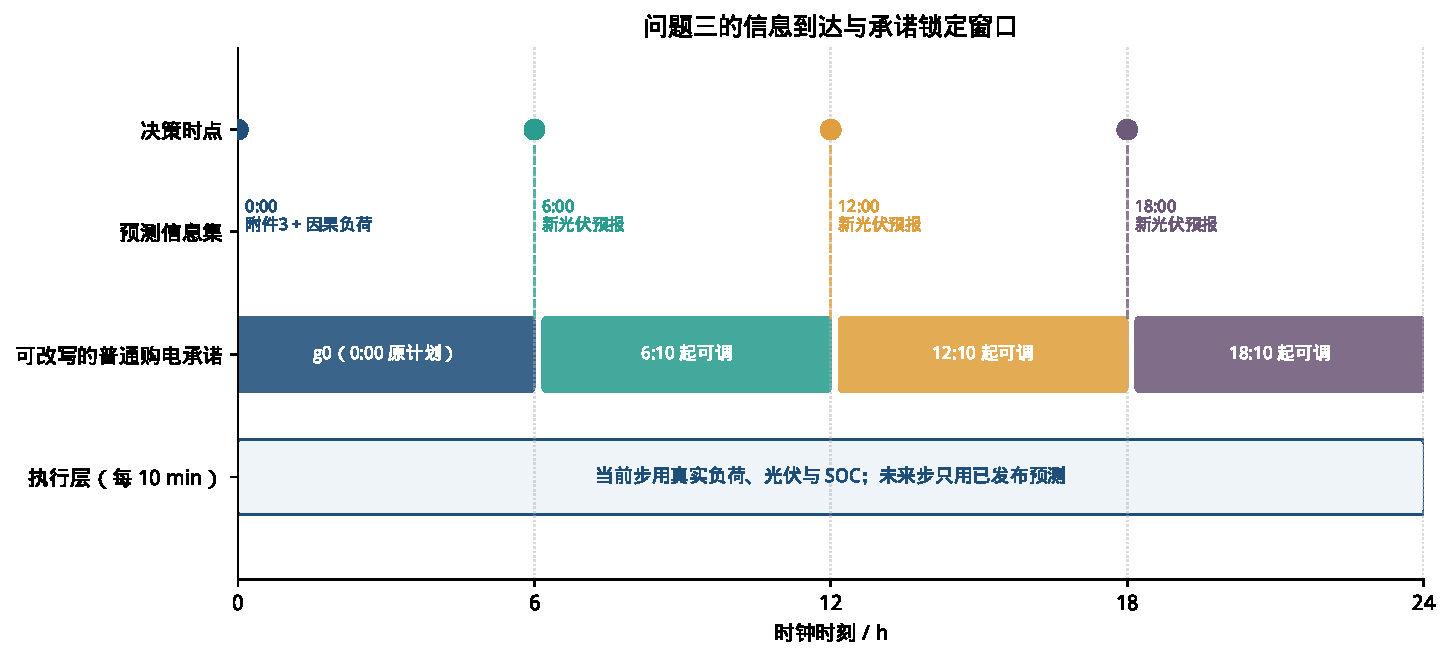
\includegraphics[width=0.95\textwidth]{../fig/q3_paper/fig3_info_timeline.pdf}
\caption{问题三的信息到达与承诺改写窗口。虚线为预测发布时间；色块表示该时点之后尚未执行、因而可以改写的普通购电承诺。执行层始终只在当前 10 分钟使用真实负荷与光伏。}
\label{fig:q3-info}
\end{figure}

\begin{figure}[H]
\centering
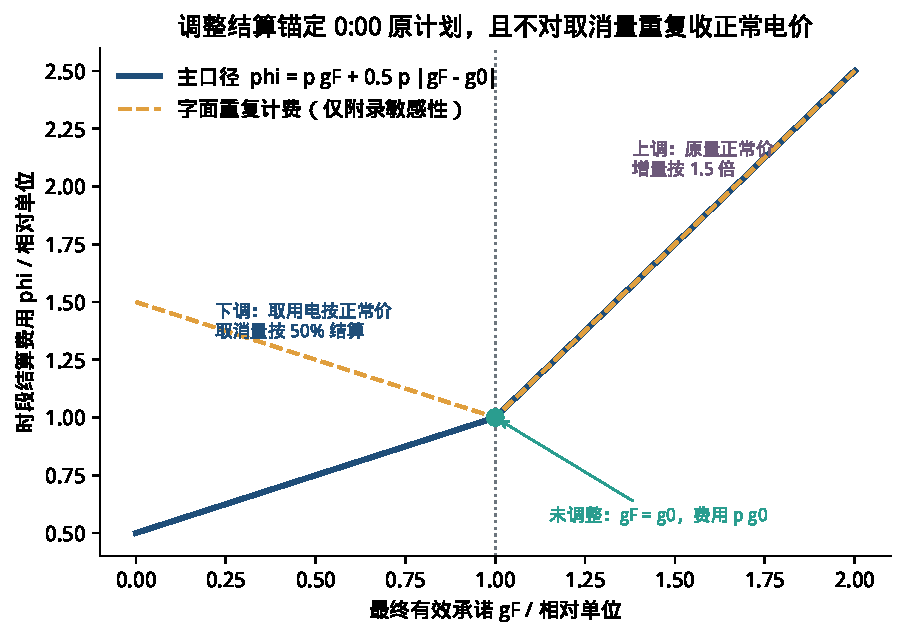
\includegraphics[width=0.72\textwidth]{../fig/q3_paper/fig3_settlement_phi.pdf}
\caption{以 0:00 原计划为锚点的调整结算。实线为主口径~\eqref{eq:q3-phi}；虚线把下调取消量同时按正常价和 50\% 计价，只作附录敏感性，以免把题意歧义写成唯一市场事实。}
\label{fig:q3-phi}
\end{figure}

\subsubsection{主模型：四时点滚动重优化}

物理可行性与问题一、问题二相同。公共母线能量平衡与 SOC 转移为
\begin{equation}
\label{eq:q3-balance}
x_{d,t}+e_{d,t}+P_{d,t}-w_{d,t}+r_{d,t}=L_{d,t}+c_{d,t},
\end{equation}
\begin{equation}
\label{eq:q3-soc}
E_{d,t}=E_{d,t-1}+\eta_c c_{d,t}-\frac{r_{d,t}}{\eta_d}.
\end{equation}
普通购电只能在当期承诺内取用，\(0\le x_{d,t}\le g_{d,t}\)；多余承诺已经按~\eqref{eq:q3-phi} 结算，但不能凭空转移到其他时段。跨时搬运只能经过“购电或光伏 \(\to\) 充电 \(\to\) SOC \(\to\) 放电”。在正电价、无上网收益且电池有损耗时，同时充放电被更低损耗的等价解支配；求解后仍审计 \(c_{d,t}r_{d,t}=0\)。

\paragraph{M0：0:00 后不调整。}
以 0:00 的 \((\widehat L,\widehat P^{0})\) 制订 \(g^{0}\)，此后强制 \(g^{F}=g^{0}\)。它回答“新预测总体上有没有货币价值”：任何允许更新的策略，必须在同一初始 SOC、同一结算和同一执行规则下给出更低的实现成本~\eqref{eq:q3-total-cost}，否则更新权利只是名义上的。

\paragraph{M1：每次更新都评估并求解。}
设更新时刻 \(\tau\) 的当前真实 SOC 为 \(E_{d,\tau}\)，更新前承诺为 \(g^{\mathrm{pre}}\)。在剩余时域 \(\mathcal T_\tau\) 上解
\begin{equation}
\label{eq:q3-m1}
\boxed{
\left\{
\begin{aligned}
\min_{g,x,e,c,r,w,E}\quad
&\sum_{t\in\mathcal T_\tau}
\bigl[\phi_t(g^{0}_{d,t},g_{d,t})+5p_t e_{d,t}\bigr]
+V_{d+1}(E_{d,144}),\\
&g_{d,t}=g^{\mathrm{pre}}_{d,t},\qquad t\notin\mathcal T_\tau,\\
&0\le x_{d,t}\le g_{d,t},\qquad g_{d,t}\ge 0,\\
&\text{以及~\eqref{eq:q3-balance}--\eqref{eq:q3-soc} 与功率、SOC、弃光边界。}
\end{aligned}
\right.}
\end{equation}
规划阶段的平衡使用 \((\widehat L_{d,t},\widehat P^{\tau}_{d,t})\)；执行当前一步时改用真实 \((L_{d,t},P_{d,t})\)，只实施本步动作，下一时段带入真实 SOC 再滚动。这不是预知未来光伏或未来负荷的事后最优。因为 \(g=g^{\mathrm{pre}}\) 始终可行，并且调整价格已经进入目标，模型只有在改计划后仍能降低预计总成本时才会离开原承诺。因而 M1 的“每次更新”是指每次都求解，而不是强迫计划变化。

\paragraph{M6：用信息价值记录是否实施调整。}
在 \(\tau\in\{6{:}00,12{:}00,18{:}00\}\) 计算
\begin{equation}
\label{eq:q3-voi}
\begin{aligned}
J^{\mathrm{fix}}_{\tau}&=\min\{J_{\tau}:g_{d,t}=g^{\mathrm{pre}}_{d,t},\ t\in\mathcal T_\tau\},\\
J^{\mathrm{free}}_{\tau}&=\min\{J_{\tau}:g_{d,t}\ge 0,\ t\in\mathcal T_\tau\},\\
VoI_{\tau}&=J^{\mathrm{fix}}_{\tau}-J^{\mathrm{free}}_{\tau}.
\end{aligned}
\end{equation}
仅当 \(VoI_{\tau}>\varepsilon\) 时写入新承诺，否则维持 \(g^{\mathrm{pre}}\)。\(\varepsilon=0.01\) 元取求解器货币容差，只防止无意义的浮点微调。当保持原承诺可行、调整费进入目标且 \(\varepsilon\to 0\) 时，M1 与 M6 给出同一经济最优解。因此 M6 不是第二个独立主算法，而是 M1 的可解释实施层：它把“新预测值不值得用”写成逐时点的 \(VoI\) 台账。真正有信息含义的比较是
\[
\text{M0},\quad
\text{M1/M6},\quad
M_{6},\ M_{12},\ M_{18},
\]
其中后三个消融各自只开放一个更新时点，用于回答哪一次预报对实现成本最关键。图~\ref{fig:q3-voi} 给出该实施逻辑。

\begin{figure}[H]
\centering
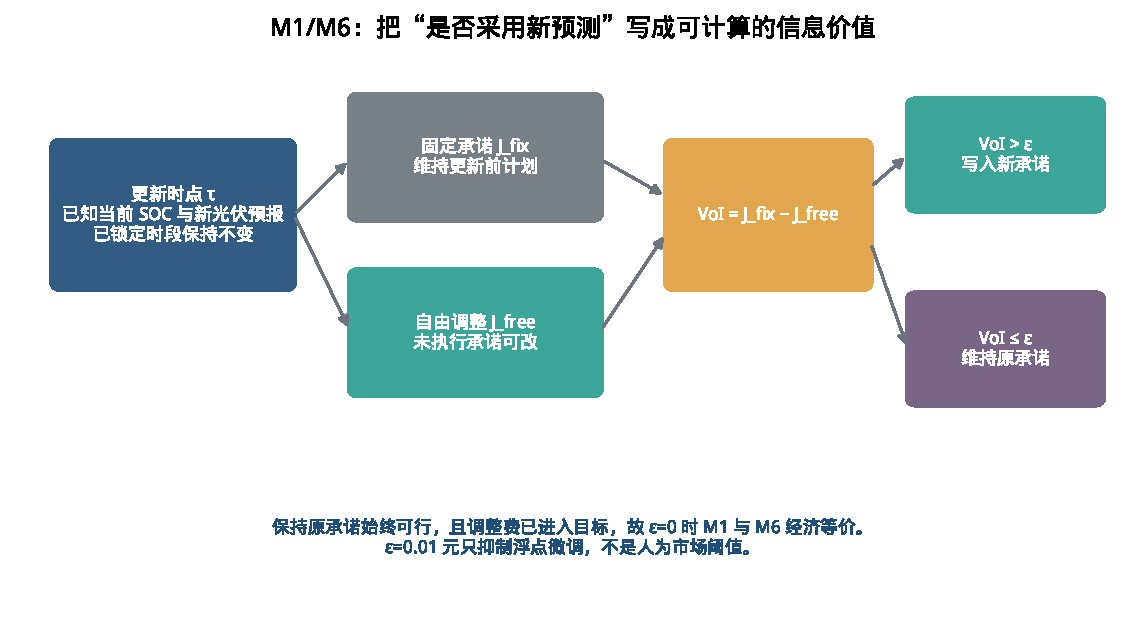
\includegraphics[width=0.92\textwidth]{../fig/q3_paper/fig3_voi_decision.pdf}
\caption{更新时点上的信息价值判定。由于不调整始终可行，\(VoI\) 不会人为制造成本差；单时点消融而不是 M1 对 M6 的成本差，才是“哪个时刻的预测值得使用”的证据。}
\label{fig:q3-voi}
\end{figure}

\paragraph{终端价值。}
日末不强制回到日初 SOC。为避免最后数小时透支电池，优化视域延长到次日，或等价加入到达项 \(V_{d+1}(E_{d,144})\)。该项与问题二政策一致方案相同：由次日基准预测 LP（而非情景全路径补救）在若干 SOC 样本上生成凸支持割，并以弦线--切面间隙作为误差证书。预测输入改用问题三的因果负荷与附件 3 更新口径。它只引导今日末库存，次日购电计划必须到次日 0:00 重新制订，不得提前写入结果文件或重复计费。

\subsubsection{求解算法}

式~\eqref{eq:q3-m1} 在固定预测轨迹下是线性规划：\(\phi_t\) 的绝对值由非负上、下调变量线性化，能量平衡与 SOC 均为线性等式，容量与功率均为盒约束。主求解使用 LP（HiGHS）；若出现数值上的同时充放电，先以最小吞吐量作词典序次目标，仅在仍不能消除时用互斥二元变量复核。选择 LP 而不是遗传算法或完整多阶段随机动态规划，是因为：题目的调整费和紧急电价已经给出可加的货币目标；承诺跨时段的耦合由 SOC 线性传递；计算瓶颈在于全年、多策略、每 10 分钟滚动，而不是非凸组合爆炸。完整情景树（规格中的 M5）能够刻画未发生光伏误差的条件残差，但要求购电承诺跨情景一致、控制动作服从信息历史，不能把每条未来轨迹的储能当作日初指令。M5 只作为不确定性扩展，不替代 M1/M6 的主结果；在其全年审计完成前，正文不把问题三称为严格多阶段随机最优控制。

算法流程如下。对每个策略、每一日：用~\eqref{eq:q3-load} 与 0:00 光伏映射形成日初信息并求解 \(g^{0}\)；在允许的更新点比较 \(J^{\mathrm{fix}}\) 与 \(J^{\mathrm{free}}\)；每个 10 分钟只执行当前动作并更新真实 SOC；日成本按~\eqref{eq:q3-total-cost} 归集。全年比较时，每个策略必须从 2025-01-01 的 6000 kWh 起沿\textbf{自身}决策连续传递 SOC，不得借用 M0 或其他策略的库存路径。1 月用于状态预热与预测历史，题设结果表覆盖 2--12 月；若报告年度成本，须写明是 1--12 月完整核算还是 2--12 月输出区间，二者不得混报。

\subsubsection{结果与机制解释}
\label{sec:q3-results}

本节数字一律待队长把因果负荷主路径写入 \texttt{results\_summary.md} 后再填。当前两日试算使用了当天完整真实负荷，只证明结算公式、锁定窗口和物理残差链路可运行，不能代表现实可执行的日前/日内策略。

待填的主比较应同时给出总成本、普通结算成本、紧急购电成本和弃光，避免把“调整次数多”直接写成“更好”。预期的机制解释（有签收数字后按实际符号改写，不得预先断言全年排序）是：允许更新的策略如果优于 M0，其来源应是\textbf{减少 5 倍紧急补购}，而普通结算成本完全可能上升——因为上调按 1.5 倍付费，模型只有在避免紧急购电的收益超过调整费时才会增加 \(g\)。单时点消融若出现“仅 6:00 更新的实现成本劣于 M0”，原因通常是过早下调后，后续真实光伏/负荷偏差无法在已锁定期内用正常购电挽回，只能转化为紧急购电或被动弃光；这恰恰说明 \(VoI\) 是当时信息下的预测收益，不是实现路径上的保证收益。18:00 更新若增量很小，则因为剩余时段短、可改电量少，且日末库存已由 48 小时到达项约束。

\begin{table}[H]
\centering
\caption{问题三主比较（因果负荷、线性锚点映射、0:00 锚定结算；数字待签收）}
\label{tab:q3-strategy}
\begin{tabular}{lcccc}
\toprule
策略 & 总成本 / 元 & 相对 M0 & 普通结算 / 元 & 紧急成本 / 元 \\
\midrule
M0（不调整） & \QThreeMZeroCost & --- & \QThreeUnsigned & \QThreeUnsigned \\
\(M_{6}\) 仅 6:00 & \QThreeUnsigned & \QThreeUnsigned & \QThreeUnsigned & \QThreeUnsigned \\
\(M_{12}\) 仅 12:00 & \QThreeUnsigned & \QThreeUnsigned & \QThreeUnsigned & \QThreeUnsigned \\
\(M_{18}\) 仅 18:00 & \QThreeUnsigned & \QThreeUnsigned & \QThreeUnsigned & \QThreeUnsigned \\
M1/M6（三点均评估） & \QThreeMainCost & \QThreeSavePct & \QThreeSettleLift & \QThreeEmergDrop \\
\bottomrule
\end{tabular}
\end{table}

指定展示日的计划购电量、调整购电量、四小时充放电与紧急购电按题设 \texttt{result3.xlsx} 列出。正文须同时说明该日 0:00 原计划、各更新点 \(VoI\) 以及调整方向，避免只贴最终 \(g^{F}\)。题设导出区间为 2025-02-01 至 2025-12-31；1 月不写入结果表，但跨日 SOC 必须从年初连续而来。

不得把问题二已签收的 2--12 月成本 14{,}456{,}670.55 元，或政策一致部署路径的 2--12 月成本，与问题三年度成本直接相减。两问结算对象不同（问题二按锁定额度 \(q\) 付费，问题三按 \(\phi(g^{0},g^{F})\) 付费），信息集也不同。对照只能在队长同时签收两问主口径、并统一首末 SOC 与核算区间之后，分项列出计划/调整/紧急三项。

\subsubsection{验证、敏感性与表述边界}

必须通过、且论文只声称“通过数值审计”的项目包括：逐 10 分钟能量平衡与 SOC 递推残差达到数值求解量级；SOC、功率、弃光边界无违例；更新点之前的 \(g\) 不被改写；\(x\le g\)；无同时充放电；\(\phi\) 对上调、下调、未调三类样本与分段定义一致；主模型对当天尚未发生的负荷做扰动时，当时计划不变。\(\texttt{actual\_load\_proxy}\) 必须单独成表，不能并入主比较。

小时预报到 10 分钟的线性锚点映射不是附件唯一规定，分段常数映射只作敏感性。主结算不是题意的唯一读法，相邻版本逐次结算只作附录。在这些全年组合跑完以前，只可以写“两日回归样本未改变审计结论”，不可以写“全年映射与结算解释下策略排序均稳健”。年末 1200 kWh 与 6000 kWh 是核算边界：前者允许释放期初库存，后者要求年末仍保留该库存；成本差应首先解释为库存会计，其次才检查是否改变策略排序。控制器能够即时获得当前负荷/光伏，是本文的控制信息假设，题目未给出通信延迟，故不把结果写成工程部署方案。

图~\ref{fig:q3-overview} 总结问题三在四问主线中的位置：它只放宽承诺改写的时点，不另起一套储能物理。

\begin{figure}[H]
\centering
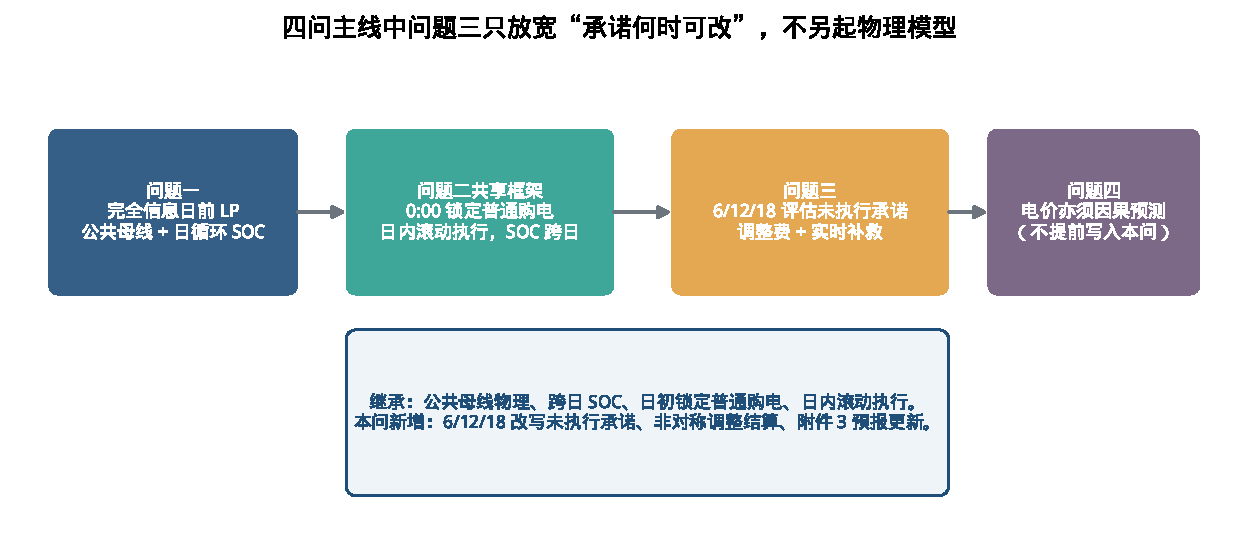
\includegraphics[width=0.96\textwidth]{../fig/q3_paper/fig3_q2_to_q3_overview.pdf}
\caption{问题三在全文主线中的位置。评委从本图应读出：储能物理连续继承，信息集按问递进；本问只放宽普通购电承诺的改写时点，并把调整费计入目标。}
\label{fig:q3-overview}
\end{figure}

% 摘要可用段落（数字仍为宏）
% \textbf{针对问题三，}由于光伏预测在 0:00、6:00、12:00、18:00 更新，若继续全日锁定普通购电，将放弃题目允许的调整权并放大紧急购电。因此以 0:00 原计划为唯一结算锚点，建立计入非对称调整费的剩余时域滚动 LP，并用预测成本差 \(VoI\) 记录是否实施调整。主方案在因果负荷与线性锚点映射下的实现成本为 \QThreeMainCost 元，相对从不调整的 M0 为 \QThreeSavePct。该差额来自紧急购电下降与普通结算变化的对冲，而不是取消调整费或预知未来实际曲线。
。

% ---------- 未核数字宏（队长写入 results_summary.md 后再替换）----------
\newcommand{\QThreeUnsigned}{[待签收]}
\newcommand{\QThreeMainCost}{\QThreeUnsigned}
\newcommand{\QThreeMZeroCost}{\QThreeUnsigned}
\newcommand{\QThreeSaveVsMZero}{\QThreeUnsigned}
\newcommand{\QThreeSavePct}{\QThreeUnsigned}
\newcommand{\QThreeEmergDrop}{\QThreeUnsigned}
\newcommand{\QThreeSettleLift}{\QThreeUnsigned}
\newcommand{\QThreeYearEndA}{1200}
\newcommand{\QThreeYearEndB}{6000}

% ============================================================
\subsection{问题三：预测更新下的购电调整与储能滚动调度}
% ============================================================

\subsubsection{问题的数学本质与同问题二的衔接}

问题三并不改写问题一、问题二已经成立的公共母线能量平衡、储能效率和跨日 SOC 传递，真正新增的困难是\textbf{信息到达方式}：每日 0:00、6:00、12:00、18:00 各得到一条未来 24 小时光伏点预测，题目允许据此调整尚未执行的购电策略，并且上调、下调分别按交易时刻电价的 1.5 倍与 50\% 结算。因此本问的对象不再是“一次性锁定的日前额度”，而是一条随预测更新而可能改写的承诺过程
\[
g^{0}_{d,\cdot}\;\longrightarrow\;
g^{\tau}_{d,\cdot}\ (\tau\in\{6{:}00,12{:}00,18{:}00\})\;\longrightarrow\;
g^{F}_{d,\cdot},
\]
其中 \(g^{F}\) 是该时段到来前最后一次有效承诺。

若把问题二的“全日锁定、日内只靠储能和紧急购电补救”原样搬来，将直接放弃题目明确给出的三次更新权利，必然高估紧急购电。反之，若在 6:00 之后仍允许改写 0:00--6:00 已经执行的电量，或把尚未发布的附件 3 预测、当天未来实际光伏当作当前决策输入，则模型在信息上优于任何可执行策略。由于问题二已经把普通购电承诺与实时物理补救分开，问题三只需在同一框架上打开放宽条件：\textbf{承诺层允许按更新时点改写未执行时段，执行层仍然只能使用已观测状态}。储能与紧急购电继续承担补救角色，不能替代本可在最近一次更新点完成的正常购电调整。

本问与问题二的衔接建立在最新政策一致设计之上：日前层只在单一因果基准预测轨迹上求线性规划，\(K=8\) 仅用于风险储备与日内残差匹配，不再给每条历史情景单独优化储能；日内仍是锁定普通购电后的滚动执行。问题三保留同一套公共母线物理与跨日 SOC，只把“全日锁定”放宽为 6:00、12:00、18:00 可改未执行承诺。已签收附件 \texttt{result2.xlsx} 目前仍是原 \(K=8\) 情景规划口径；政策一致路径是否替换该正式文件由队长决定，\textbf{不改变}本节的结算、更新窗口和滚动 LP。

负荷预测方面，问题三固定采用透明基线 \(m_1\)：最近至多 4 个同星期历史日逐时段均值，记为 \(\widehat L_{d,t}\)。政策一致全年部署路径在 2--12 月有 207/334 日选用 \(m_3\)、56 日选用 \(m_2\)，仅 71 日为 \(m_1\)，因此二者只是结构同类，\textbf{不是同一预测器}；问题三也不随问题二每 14 日在线切换。48 小时终端价值与新问题二一致，由次日基准预测 LP 的支持割近似，数值必须按附件 3 的更新口径重新估计，不得搬用问题二的切面，也不得再写成旧方案的“全路径情景储能补救”。

\subsubsection{符号、信息集与调整结算}

一天划分为 \(T=144\) 个 10 分钟时段，\(\Delta t=1/6\) h。附件 2 的功率先化为时段能量 \(L_{d,t}=\ell_{d,t}\Delta t\)、\(P_{d,t}=\rho_{d,t}\Delta t\)。更新时点集合为 \(\mathcal U=\{0{:}00,6{:}00,12{:}00,18{:}00\}\)。令 \(\mathcal T_\tau\) 为 \(\tau\) 之后当日尚未执行的时段；6:00、12:00、18:00 的首个可改时段分别为 6:10、12:10、18:10。

\begin{table}[H]
\centering
\caption{问题三新增或含义发生变化的主要符号}
\label{tab:q3-symbols}
\small
\begin{tabular}{cll}
\toprule
符号 & 含义 & 单位 / 边界 \\
\midrule
\(g^{0}_{d,t}\) & 当日 0:00 制订的普通购电原计划 & kWh，\(g^{0}\ge 0\) \\
\(g_{d,t}\) & 当前版本承诺；时段到来前的最终值为 \(g^{F}_{d,t}\) & kWh，\(g\ge 0\) \\
\(x_{d,t}\) & 从当期承诺中实际取用的普通电量 & \(0\le x\le g^{F}\) \\
\(e_{d,t}\) & 实时紧急购电 & kWh，\(e\ge 0\) \\
\(\phi_t(g^{0},g^{F})\) & 相对 0:00 原计划的计划--调整结算 & 元 \\
\(\widehat P^{\tau}_{d,t}\) & 时点 \(\tau\) 发布后映射得到的 10 分钟光伏预测 & kWh \\
\(\widehat L_{d,t}\) & 日初因果负荷预测（执行前缀外保持不变） & kWh \\
\(VoI_{\tau}\) & 时点 \(\tau\) 上“允许调整”相对“维持承诺”的预测成本差 & 元 \\
\(V_{d+1}(E_{d,144})\) & 下一日 SOC 的虚拟到达成本，不计入当日账单 & 元 \\
\bottomrule
\end{tabular}
\end{table}

充放电 \(c_{d,t},r_{d,t}\)、弃光 \(w_{d,t}\) 与 SOC \(E_{d,t}\) 沿用问题一的公共母线口径：功率上限 \(5000\Delta t\) kWh，SOC 窗口 \([1200,10800]\) kWh，\(\eta_c=\eta_d=\sqrt{0.9}\)，\(E_{2025\text{-}01\text{-}01,0}=6000\) kWh，且 \(E_{d+1,0}=E_{d,144}\)。已签收问题二与政策一致全年部署路径均在 2025-12-31 日末落到 \(1200\) kWh，故主核算取年末 \(E_{\mathrm{end}}=\QThreeYearEndA\) kWh，作为与问题二可比的统一库存边界；\(\QThreeYearEndB\) kWh 仅作库存中性敏感性。该选择不是题面规定，也不是社区运行规律。2 月初库存两条问题二路径并不相同（已签收约 \(2645\) kWh，政策一致部署约 \(1228\) kWh），问题三必须从 1 月 1 日 \(6000\) kWh 沿自身决策传递 SOC，不得借用问题二的 2 月 1 日状态。

\paragraph{主结算口径。}
题目同时出现“原计划高于调整量按 50\% 结算、调整量高于原计划按 1.5 倍结算”。若把“原计划的正常电费”与“下调违约费”对取消量同时全额累加，取消部分会被收一次正常价再收一次 50\% 价。经济上可执行、且不重复计价的读法是：最终实际采购的 \(g^{F}\) 按正常价结算，相对 \(g^{0}\) 的偏差按半价的绝对值附加。于是
\begin{equation}
\label{eq:q3-phi}
\phi_t(g^{0},g^{F})=p_t g^{F}+\frac12 p_t\lvert g^{F}-g^{0}\rvert
=
\begin{cases}
p_t g^{F}+\dfrac12 p_t(g^{0}-g^{F}), & g^{F}\le g^{0},\\[4pt]
p_t g^{0}+\dfrac32 p_t(g^{F}-g^{0}), & g^{F}>g^{0}.
\end{cases}
\end{equation}
同一时段可能在 6:00、12:00、18:00 被多次讨论，但账单始终锚定该日 0:00 的 \(g^{0}\)，不对未执行的中间版本逐笔叠加。式~\eqref{eq:q3-phi} 是本文对题意的主解释，不是市场规则的唯一数学定理；相邻版本逐次结算只进入附录敏感性，不进入主结论。

目标是最小化实际发生的购电成本
\begin{equation}
\label{eq:q3-total-cost}
\min C=\sum_{d,t}\Bigl[\phi_t\bigl(g^{0}_{d,t},g^{F}_{d,t}\bigr)+5p_t e_{d,t}\Bigr],
\end{equation}
而不是最小化某一次计划量。\(V_{d+1}\) 只出现在滚动优化的目标中，用于避免有限视域末端把电池不合理地耗尽，不计入~\eqref{eq:q3-total-cost}。

\paragraph{因果预测。}
附件 3 给出逐小时光伏点预测。每次更新以\textbf{该时点刚观测到的实际光伏}为锚点，再与随后 24 个整点预报线性插值到 10 分钟网格，得到 \(\widehat P^{\tau}\)。不得使用未来附件 2 实际光伏做插值节点。负荷没有单独预报附件：主模型对计划日 \(d\) 取
\begin{equation}
\label{eq:q3-load}
\widehat L_{d,t}=\frac1{|\mathcal H_d|}\sum_{j\in\mathcal H_d}L_{j,t},
\end{equation}
其中 \(\mathcal H_d\) 是日期严格早于 \(d\) 的最近至多 4 个同星期历史日。6:00/12:00/18:00 规划未来时段时仍使用该日 0:00 已形成的 \(\widehat L\)，不读取当天尚未发生的附件 2 负荷。每 10 分钟执行当前一步时，才以当期真实 \((L_{d,t},P_{d,t})\) 闭合能量平衡。附件 2 当日完整负荷曲线仅作为理想化对照 \(\texttt{actual\_load\_proxy}\)，用于量化“若负荷被完美预知”的信息价值，不得作为主方案或可执行策略。

图~\ref{fig:q3-info} 给出承诺锁定窗口与信息集；图~\ref{fig:q3-phi} 给出主结算与重复计费读法的对比。

\begin{figure}[H]
\centering
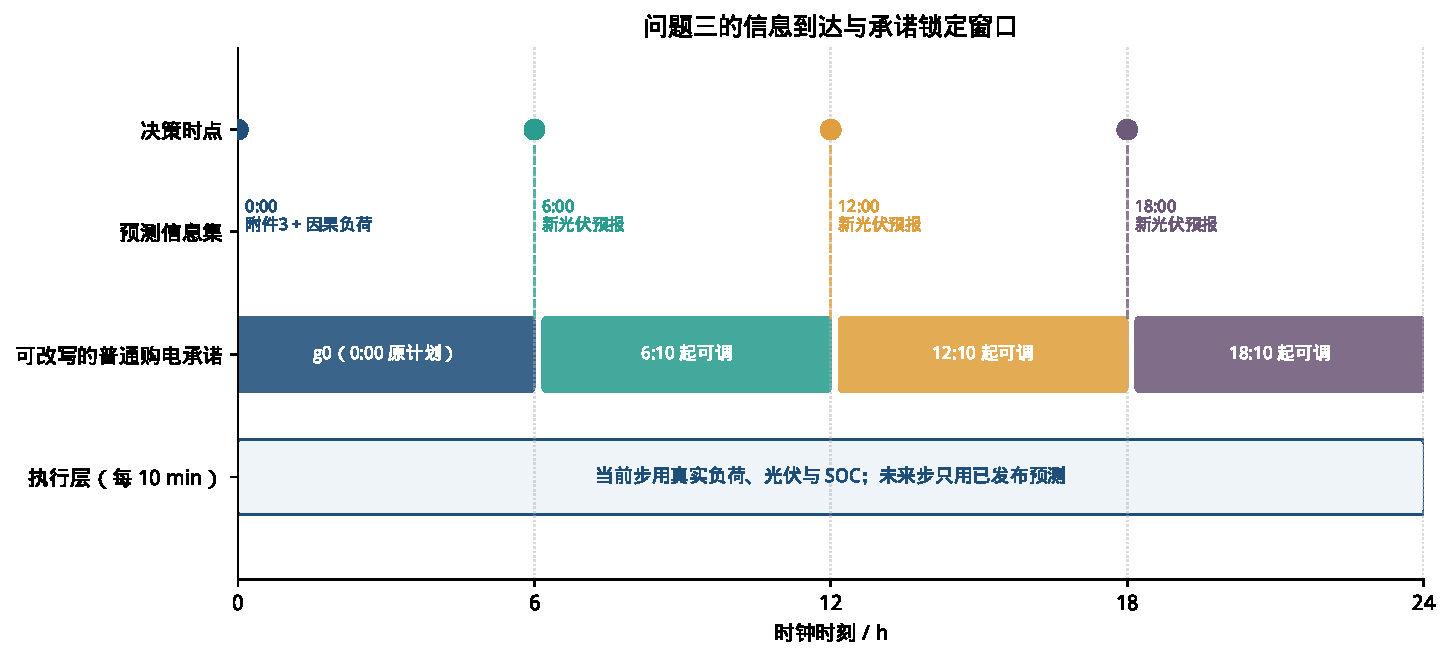
\includegraphics[width=0.95\textwidth]{../fig/q3_paper/fig3_info_timeline.pdf}
\caption{问题三的信息到达与承诺改写窗口。虚线为预测发布时间；色块表示该时点之后尚未执行、因而可以改写的普通购电承诺。执行层始终只在当前 10 分钟使用真实负荷与光伏。}
\label{fig:q3-info}
\end{figure}

\begin{figure}[H]
\centering
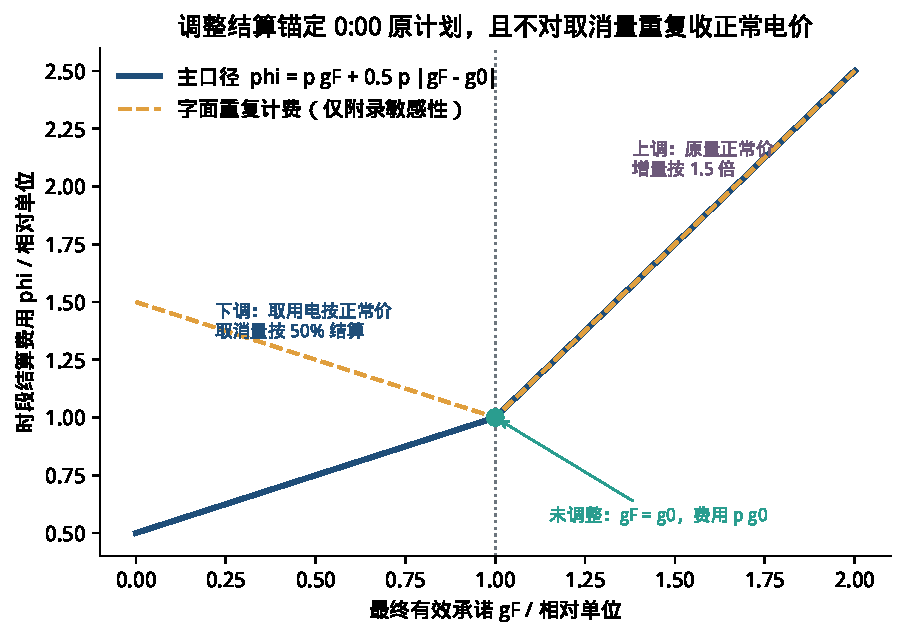
\includegraphics[width=0.72\textwidth]{../fig/q3_paper/fig3_settlement_phi.pdf}
\caption{以 0:00 原计划为锚点的调整结算。实线为主口径~\eqref{eq:q3-phi}；虚线把下调取消量同时按正常价和 50\% 计价，只作附录敏感性，以免把题意歧义写成唯一市场事实。}
\label{fig:q3-phi}
\end{figure}

\subsubsection{主模型：四时点滚动重优化}

物理可行性与问题一、问题二相同。公共母线能量平衡与 SOC 转移为
\begin{equation}
\label{eq:q3-balance}
x_{d,t}+e_{d,t}+P_{d,t}-w_{d,t}+r_{d,t}=L_{d,t}+c_{d,t},
\end{equation}
\begin{equation}
\label{eq:q3-soc}
E_{d,t}=E_{d,t-1}+\eta_c c_{d,t}-\frac{r_{d,t}}{\eta_d}.
\end{equation}
普通购电只能在当期承诺内取用，\(0\le x_{d,t}\le g_{d,t}\)；多余承诺已经按~\eqref{eq:q3-phi} 结算，但不能凭空转移到其他时段。跨时搬运只能经过“购电或光伏 \(\to\) 充电 \(\to\) SOC \(\to\) 放电”。在正电价、无上网收益且电池有损耗时，同时充放电被更低损耗的等价解支配；求解后仍审计 \(c_{d,t}r_{d,t}=0\)。

\paragraph{M0：0:00 后不调整。}
以 0:00 的 \((\widehat L,\widehat P^{0})\) 制订 \(g^{0}\)，此后强制 \(g^{F}=g^{0}\)。它回答“新预测总体上有没有货币价值”：任何允许更新的策略，必须在同一初始 SOC、同一结算和同一执行规则下给出更低的实现成本~\eqref{eq:q3-total-cost}，否则更新权利只是名义上的。

\paragraph{M1：每次更新都评估并求解。}
设更新时刻 \(\tau\) 的当前真实 SOC 为 \(E_{d,\tau}\)，更新前承诺为 \(g^{\mathrm{pre}}\)。在剩余时域 \(\mathcal T_\tau\) 上解
\begin{equation}
\label{eq:q3-m1}
\boxed{
\left\{
\begin{aligned}
\min_{g,x,e,c,r,w,E}\quad
&\sum_{t\in\mathcal T_\tau}
\bigl[\phi_t(g^{0}_{d,t},g_{d,t})+5p_t e_{d,t}\bigr]
+V_{d+1}(E_{d,144}),\\
&g_{d,t}=g^{\mathrm{pre}}_{d,t},\qquad t\notin\mathcal T_\tau,\\
&0\le x_{d,t}\le g_{d,t},\qquad g_{d,t}\ge 0,\\
&\text{以及~\eqref{eq:q3-balance}--\eqref{eq:q3-soc} 与功率、SOC、弃光边界。}
\end{aligned}
\right.}
\end{equation}
规划阶段的平衡使用 \((\widehat L_{d,t},\widehat P^{\tau}_{d,t})\)；执行当前一步时改用真实 \((L_{d,t},P_{d,t})\)，只实施本步动作，下一时段带入真实 SOC 再滚动。这不是预知未来光伏或未来负荷的事后最优。因为 \(g=g^{\mathrm{pre}}\) 始终可行，并且调整价格已经进入目标，模型只有在改计划后仍能降低预计总成本时才会离开原承诺。因而 M1 的“每次更新”是指每次都求解，而不是强迫计划变化。

\paragraph{M6：用信息价值记录是否实施调整。}
在 \(\tau\in\{6{:}00,12{:}00,18{:}00\}\) 计算
\begin{equation}
\label{eq:q3-voi}
\begin{aligned}
J^{\mathrm{fix}}_{\tau}&=\min\{J_{\tau}:g_{d,t}=g^{\mathrm{pre}}_{d,t},\ t\in\mathcal T_\tau\},\\
J^{\mathrm{free}}_{\tau}&=\min\{J_{\tau}:g_{d,t}\ge 0,\ t\in\mathcal T_\tau\},\\
VoI_{\tau}&=J^{\mathrm{fix}}_{\tau}-J^{\mathrm{free}}_{\tau}.
\end{aligned}
\end{equation}
仅当 \(VoI_{\tau}>\varepsilon\) 时写入新承诺，否则维持 \(g^{\mathrm{pre}}\)。\(\varepsilon=0.01\) 元取求解器货币容差，只防止无意义的浮点微调。当保持原承诺可行、调整费进入目标且 \(\varepsilon\to 0\) 时，M1 与 M6 给出同一经济最优解。因此 M6 不是第二个独立主算法，而是 M1 的可解释实施层：它把“新预测值不值得用”写成逐时点的 \(VoI\) 台账。真正有信息含义的比较是
\[
\text{M0},\quad
\text{M1/M6},\quad
M_{6},\ M_{12},\ M_{18},
\]
其中后三个消融各自只开放一个更新时点，用于回答哪一次预报对实现成本最关键。图~\ref{fig:q3-voi} 给出该实施逻辑。

\begin{figure}[H]
\centering
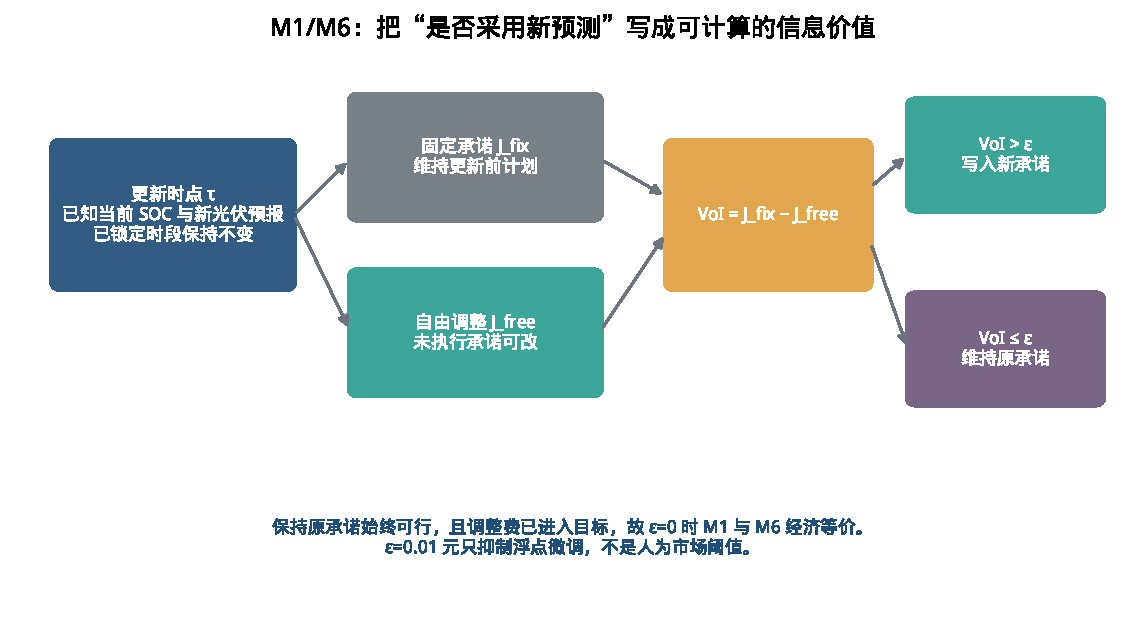
\includegraphics[width=0.92\textwidth]{../fig/q3_paper/fig3_voi_decision.pdf}
\caption{更新时点上的信息价值判定。由于不调整始终可行，\(VoI\) 不会人为制造成本差；单时点消融而不是 M1 对 M6 的成本差，才是“哪个时刻的预测值得使用”的证据。}
\label{fig:q3-voi}
\end{figure}

\paragraph{终端价值。}
日末不强制回到日初 SOC。为避免最后数小时透支电池，优化视域延长到次日，或等价加入到达项 \(V_{d+1}(E_{d,144})\)。该项与问题二政策一致方案相同：由次日基准预测 LP（而非情景全路径补救）在若干 SOC 样本上生成凸支持割，并以弦线--切面间隙作为误差证书。预测输入改用问题三的因果负荷与附件 3 更新口径。它只引导今日末库存，次日购电计划必须到次日 0:00 重新制订，不得提前写入结果文件或重复计费。

\subsubsection{求解算法}

式~\eqref{eq:q3-m1} 在固定预测轨迹下是线性规划：\(\phi_t\) 的绝对值由非负上、下调变量线性化，能量平衡与 SOC 均为线性等式，容量与功率均为盒约束。主求解使用 LP（HiGHS）；若出现数值上的同时充放电，先以最小吞吐量作词典序次目标，仅在仍不能消除时用互斥二元变量复核。选择 LP 而不是遗传算法或完整多阶段随机动态规划，是因为：题目的调整费和紧急电价已经给出可加的货币目标；承诺跨时段的耦合由 SOC 线性传递；计算瓶颈在于全年、多策略、每 10 分钟滚动，而不是非凸组合爆炸。完整情景树（规格中的 M5）能够刻画未发生光伏误差的条件残差，但要求购电承诺跨情景一致、控制动作服从信息历史，不能把每条未来轨迹的储能当作日初指令。M5 只作为不确定性扩展，不替代 M1/M6 的主结果；在其全年审计完成前，正文不把问题三称为严格多阶段随机最优控制。

算法流程如下。对每个策略、每一日：用~\eqref{eq:q3-load} 与 0:00 光伏映射形成日初信息并求解 \(g^{0}\)；在允许的更新点比较 \(J^{\mathrm{fix}}\) 与 \(J^{\mathrm{free}}\)；每个 10 分钟只执行当前动作并更新真实 SOC；日成本按~\eqref{eq:q3-total-cost} 归集。全年比较时，每个策略必须从 2025-01-01 的 6000 kWh 起沿\textbf{自身}决策连续传递 SOC，不得借用 M0 或其他策略的库存路径。1 月用于状态预热与预测历史，题设结果表覆盖 2--12 月；若报告年度成本，须写明是 1--12 月完整核算还是 2--12 月输出区间，二者不得混报。

\subsubsection{结果与机制解释}
\label{sec:q3-results}

本节数字一律待队长把因果负荷主路径写入 \texttt{results\_summary.md} 后再填。当前两日试算使用了当天完整真实负荷，只证明结算公式、锁定窗口和物理残差链路可运行，不能代表现实可执行的日前/日内策略。

待填的主比较应同时给出总成本、普通结算成本、紧急购电成本和弃光，避免把“调整次数多”直接写成“更好”。预期的机制解释（有签收数字后按实际符号改写，不得预先断言全年排序）是：允许更新的策略如果优于 M0，其来源应是\textbf{减少 5 倍紧急补购}，而普通结算成本完全可能上升——因为上调按 1.5 倍付费，模型只有在避免紧急购电的收益超过调整费时才会增加 \(g\)。单时点消融若出现“仅 6:00 更新的实现成本劣于 M0”，原因通常是过早下调后，后续真实光伏/负荷偏差无法在已锁定期内用正常购电挽回，只能转化为紧急购电或被动弃光；这恰恰说明 \(VoI\) 是当时信息下的预测收益，不是实现路径上的保证收益。18:00 更新若增量很小，则因为剩余时段短、可改电量少，且日末库存已由 48 小时到达项约束。

\begin{table}[H]
\centering
\caption{问题三主比较（因果负荷、线性锚点映射、0:00 锚定结算；数字待签收）}
\label{tab:q3-strategy}
\begin{tabular}{lcccc}
\toprule
策略 & 总成本 / 元 & 相对 M0 & 普通结算 / 元 & 紧急成本 / 元 \\
\midrule
M0（不调整） & \QThreeMZeroCost & --- & \QThreeUnsigned & \QThreeUnsigned \\
\(M_{6}\) 仅 6:00 & \QThreeUnsigned & \QThreeUnsigned & \QThreeUnsigned & \QThreeUnsigned \\
\(M_{12}\) 仅 12:00 & \QThreeUnsigned & \QThreeUnsigned & \QThreeUnsigned & \QThreeUnsigned \\
\(M_{18}\) 仅 18:00 & \QThreeUnsigned & \QThreeUnsigned & \QThreeUnsigned & \QThreeUnsigned \\
M1/M6（三点均评估） & \QThreeMainCost & \QThreeSavePct & \QThreeSettleLift & \QThreeEmergDrop \\
\bottomrule
\end{tabular}
\end{table}

指定展示日的计划购电量、调整购电量、四小时充放电与紧急购电按题设 \texttt{result3.xlsx} 列出。正文须同时说明该日 0:00 原计划、各更新点 \(VoI\) 以及调整方向，避免只贴最终 \(g^{F}\)。题设导出区间为 2025-02-01 至 2025-12-31；1 月不写入结果表，但跨日 SOC 必须从年初连续而来。

不得把问题二已签收的 2--12 月成本 14{,}456{,}670.55 元，或政策一致部署路径的 2--12 月成本，与问题三年度成本直接相减。两问结算对象不同（问题二按锁定额度 \(q\) 付费，问题三按 \(\phi(g^{0},g^{F})\) 付费），信息集也不同。对照只能在队长同时签收两问主口径、并统一首末 SOC 与核算区间之后，分项列出计划/调整/紧急三项。

\subsubsection{验证、敏感性与表述边界}

必须通过、且论文只声称“通过数值审计”的项目包括：逐 10 分钟能量平衡与 SOC 递推残差达到数值求解量级；SOC、功率、弃光边界无违例；更新点之前的 \(g\) 不被改写；\(x\le g\)；无同时充放电；\(\phi\) 对上调、下调、未调三类样本与分段定义一致；主模型对当天尚未发生的负荷做扰动时，当时计划不变。\(\texttt{actual\_load\_proxy}\) 必须单独成表，不能并入主比较。

小时预报到 10 分钟的线性锚点映射不是附件唯一规定，分段常数映射只作敏感性。主结算不是题意的唯一读法，相邻版本逐次结算只作附录。在这些全年组合跑完以前，只可以写“两日回归样本未改变审计结论”，不可以写“全年映射与结算解释下策略排序均稳健”。年末 1200 kWh 与 6000 kWh 是核算边界：前者允许释放期初库存，后者要求年末仍保留该库存；成本差应首先解释为库存会计，其次才检查是否改变策略排序。控制器能够即时获得当前负荷/光伏，是本文的控制信息假设，题目未给出通信延迟，故不把结果写成工程部署方案。

图~\ref{fig:q3-overview} 总结问题三在四问主线中的位置：它只放宽承诺改写的时点，不另起一套储能物理。

\begin{figure}[H]
\centering
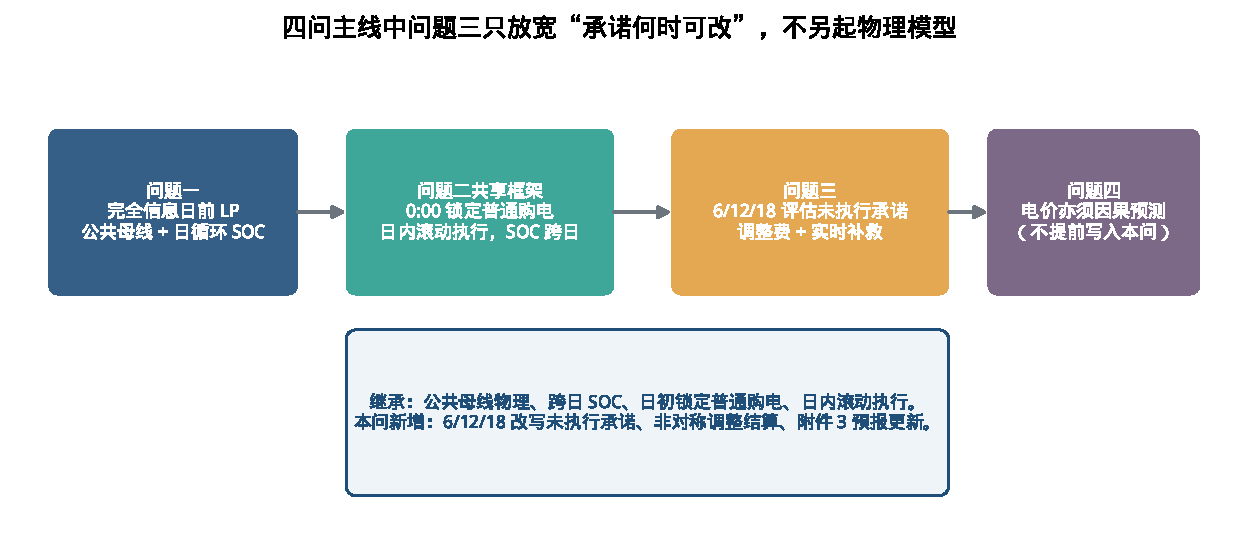
\includegraphics[width=0.96\textwidth]{../fig/q3_paper/fig3_q2_to_q3_overview.pdf}
\caption{问题三在全文主线中的位置。评委从本图应读出：储能物理连续继承，信息集按问递进；本问只放宽普通购电承诺的改写时点，并把调整费计入目标。}
\label{fig:q3-overview}
\end{figure}

% 摘要可用段落（数字仍为宏）
% \textbf{针对问题三，}由于光伏预测在 0:00、6:00、12:00、18:00 更新，若继续全日锁定普通购电，将放弃题目允许的调整权并放大紧急购电。因此以 0:00 原计划为唯一结算锚点，建立计入非对称调整费的剩余时域滚动 LP，并用预测成本差 \(VoI\) 记录是否实施调整。主方案在因果负荷与线性锚点映射下的实现成本为 \QThreeMainCost 元，相对从不调整的 M0 为 \QThreeSavePct。该差额来自紧急购电下降与普通结算变化的对冲，而不是取消调整费或预知未来实际曲线。
。

% ---------- 未核数字宏（队长写入 results_summary.md 后再替换）----------
\newcommand{\QThreeUnsigned}{[待签收]}
\newcommand{\QThreeMainCost}{\QThreeUnsigned}
\newcommand{\QThreeMZeroCost}{\QThreeUnsigned}
\newcommand{\QThreeSaveVsMZero}{\QThreeUnsigned}
\newcommand{\QThreeSavePct}{\QThreeUnsigned}
\newcommand{\QThreeEmergDrop}{\QThreeUnsigned}
\newcommand{\QThreeSettleLift}{\QThreeUnsigned}
\newcommand{\QThreeYearEndA}{1200}
\newcommand{\QThreeYearEndB}{6000}

% ============================================================
\subsection{问题三：预测更新下的购电调整与储能滚动调度}
% ============================================================

\subsubsection{问题的数学本质与同问题二的衔接}

问题三并不改写问题一、问题二已经成立的公共母线能量平衡、储能效率和跨日 SOC 传递，真正新增的困难是\textbf{信息到达方式}：每日 0:00、6:00、12:00、18:00 各得到一条未来 24 小时光伏点预测，题目允许据此调整尚未执行的购电策略，并且上调、下调分别按交易时刻电价的 1.5 倍与 50\% 结算。因此本问的对象不再是“一次性锁定的日前额度”，而是一条随预测更新而可能改写的承诺过程
\[
g^{0}_{d,\cdot}\;\longrightarrow\;
g^{\tau}_{d,\cdot}\ (\tau\in\{6{:}00,12{:}00,18{:}00\})\;\longrightarrow\;
g^{F}_{d,\cdot},
\]
其中 \(g^{F}\) 是该时段到来前最后一次有效承诺。

若把问题二的“全日锁定、日内只靠储能和紧急购电补救”原样搬来，将直接放弃题目明确给出的三次更新权利，必然高估紧急购电。反之，若在 6:00 之后仍允许改写 0:00--6:00 已经执行的电量，或把尚未发布的附件 3 预测、当天未来实际光伏当作当前决策输入，则模型在信息上优于任何可执行策略。由于问题二已经把普通购电承诺与实时物理补救分开，问题三只需在同一框架上打开放宽条件：\textbf{承诺层允许按更新时点改写未执行时段，执行层仍然只能使用已观测状态}。储能与紧急购电继续承担补救角色，不能替代本可在最近一次更新点完成的正常购电调整。

本问与问题二的衔接建立在最新政策一致设计之上：日前层只在单一因果基准预测轨迹上求线性规划，\(K=8\) 仅用于风险储备与日内残差匹配，不再给每条历史情景单独优化储能；日内仍是锁定普通购电后的滚动执行。问题三保留同一套公共母线物理与跨日 SOC，只把“全日锁定”放宽为 6:00、12:00、18:00 可改未执行承诺。已签收附件 \texttt{result2.xlsx} 目前仍是原 \(K=8\) 情景规划口径；政策一致路径是否替换该正式文件由队长决定，\textbf{不改变}本节的结算、更新窗口和滚动 LP。

负荷预测方面，问题三固定采用透明基线 \(m_1\)：最近至多 4 个同星期历史日逐时段均值，记为 \(\widehat L_{d,t}\)。政策一致全年部署路径在 2--12 月有 207/334 日选用 \(m_3\)、56 日选用 \(m_2\)，仅 71 日为 \(m_1\)，因此二者只是结构同类，\textbf{不是同一预测器}；问题三也不随问题二每 14 日在线切换。48 小时终端价值与新问题二一致，由次日基准预测 LP 的支持割近似，数值必须按附件 3 的更新口径重新估计，不得搬用问题二的切面，也不得再写成旧方案的“全路径情景储能补救”。

\subsubsection{符号、信息集与调整结算}

一天划分为 \(T=144\) 个 10 分钟时段，\(\Delta t=1/6\) h。附件 2 的功率先化为时段能量 \(L_{d,t}=\ell_{d,t}\Delta t\)、\(P_{d,t}=\rho_{d,t}\Delta t\)。更新时点集合为 \(\mathcal U=\{0{:}00,6{:}00,12{:}00,18{:}00\}\)。令 \(\mathcal T_\tau\) 为 \(\tau\) 之后当日尚未执行的时段；6:00、12:00、18:00 的首个可改时段分别为 6:10、12:10、18:10。

\begin{table}[H]
\centering
\caption{问题三新增或含义发生变化的主要符号}
\label{tab:q3-symbols}
\small
\begin{tabular}{cll}
\toprule
符号 & 含义 & 单位 / 边界 \\
\midrule
\(g^{0}_{d,t}\) & 当日 0:00 制订的普通购电原计划 & kWh，\(g^{0}\ge 0\) \\
\(g_{d,t}\) & 当前版本承诺；时段到来前的最终值为 \(g^{F}_{d,t}\) & kWh，\(g\ge 0\) \\
\(x_{d,t}\) & 从当期承诺中实际取用的普通电量 & \(0\le x\le g^{F}\) \\
\(e_{d,t}\) & 实时紧急购电 & kWh，\(e\ge 0\) \\
\(\phi_t(g^{0},g^{F})\) & 相对 0:00 原计划的计划--调整结算 & 元 \\
\(\widehat P^{\tau}_{d,t}\) & 时点 \(\tau\) 发布后映射得到的 10 分钟光伏预测 & kWh \\
\(\widehat L_{d,t}\) & 日初因果负荷预测（执行前缀外保持不变） & kWh \\
\(VoI_{\tau}\) & 时点 \(\tau\) 上“允许调整”相对“维持承诺”的预测成本差 & 元 \\
\(V_{d+1}(E_{d,144})\) & 下一日 SOC 的虚拟到达成本，不计入当日账单 & 元 \\
\bottomrule
\end{tabular}
\end{table}

充放电 \(c_{d,t},r_{d,t}\)、弃光 \(w_{d,t}\) 与 SOC \(E_{d,t}\) 沿用问题一的公共母线口径：功率上限 \(5000\Delta t\) kWh，SOC 窗口 \([1200,10800]\) kWh，\(\eta_c=\eta_d=\sqrt{0.9}\)，\(E_{2025\text{-}01\text{-}01,0}=6000\) kWh，且 \(E_{d+1,0}=E_{d,144}\)。已签收问题二与政策一致全年部署路径均在 2025-12-31 日末落到 \(1200\) kWh，故主核算取年末 \(E_{\mathrm{end}}=\QThreeYearEndA\) kWh，作为与问题二可比的统一库存边界；\(\QThreeYearEndB\) kWh 仅作库存中性敏感性。该选择不是题面规定，也不是社区运行规律。2 月初库存两条问题二路径并不相同（已签收约 \(2645\) kWh，政策一致部署约 \(1228\) kWh），问题三必须从 1 月 1 日 \(6000\) kWh 沿自身决策传递 SOC，不得借用问题二的 2 月 1 日状态。

\paragraph{主结算口径。}
题目同时出现“原计划高于调整量按 50\% 结算、调整量高于原计划按 1.5 倍结算”。若把“原计划的正常电费”与“下调违约费”对取消量同时全额累加，取消部分会被收一次正常价再收一次 50\% 价。经济上可执行、且不重复计价的读法是：最终实际采购的 \(g^{F}\) 按正常价结算，相对 \(g^{0}\) 的偏差按半价的绝对值附加。于是
\begin{equation}
\label{eq:q3-phi}
\phi_t(g^{0},g^{F})=p_t g^{F}+\frac12 p_t\lvert g^{F}-g^{0}\rvert
=
\begin{cases}
p_t g^{F}+\dfrac12 p_t(g^{0}-g^{F}), & g^{F}\le g^{0},\\[4pt]
p_t g^{0}+\dfrac32 p_t(g^{F}-g^{0}), & g^{F}>g^{0}.
\end{cases}
\end{equation}
同一时段可能在 6:00、12:00、18:00 被多次讨论，但账单始终锚定该日 0:00 的 \(g^{0}\)，不对未执行的中间版本逐笔叠加。式~\eqref{eq:q3-phi} 是本文对题意的主解释，不是市场规则的唯一数学定理；相邻版本逐次结算只进入附录敏感性，不进入主结论。

目标是最小化实际发生的购电成本
\begin{equation}
\label{eq:q3-total-cost}
\min C=\sum_{d,t}\Bigl[\phi_t\bigl(g^{0}_{d,t},g^{F}_{d,t}\bigr)+5p_t e_{d,t}\Bigr],
\end{equation}
而不是最小化某一次计划量。\(V_{d+1}\) 只出现在滚动优化的目标中，用于避免有限视域末端把电池不合理地耗尽，不计入~\eqref{eq:q3-total-cost}。

\paragraph{因果预测。}
附件 3 给出逐小时光伏点预测。每次更新以\textbf{该时点刚观测到的实际光伏}为锚点，再与随后 24 个整点预报线性插值到 10 分钟网格，得到 \(\widehat P^{\tau}\)。不得使用未来附件 2 实际光伏做插值节点。负荷没有单独预报附件：主模型对计划日 \(d\) 取
\begin{equation}
\label{eq:q3-load}
\widehat L_{d,t}=\frac1{|\mathcal H_d|}\sum_{j\in\mathcal H_d}L_{j,t},
\end{equation}
其中 \(\mathcal H_d\) 是日期严格早于 \(d\) 的最近至多 4 个同星期历史日。6:00/12:00/18:00 规划未来时段时仍使用该日 0:00 已形成的 \(\widehat L\)，不读取当天尚未发生的附件 2 负荷。每 10 分钟执行当前一步时，才以当期真实 \((L_{d,t},P_{d,t})\) 闭合能量平衡。附件 2 当日完整负荷曲线仅作为理想化对照 \(\texttt{actual\_load\_proxy}\)，用于量化“若负荷被完美预知”的信息价值，不得作为主方案或可执行策略。

图~\ref{fig:q3-info} 给出承诺锁定窗口与信息集；图~\ref{fig:q3-phi} 给出主结算与重复计费读法的对比。

\begin{figure}[H]
\centering
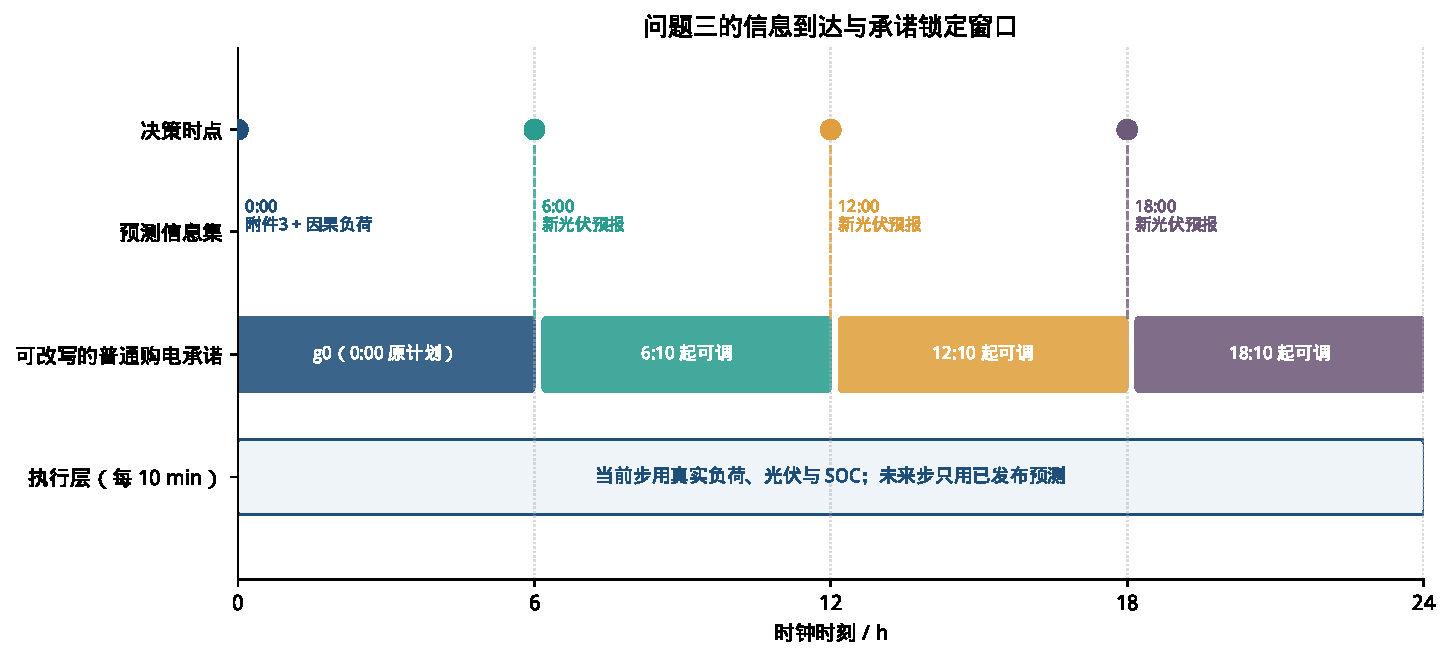
\includegraphics[width=0.95\textwidth]{../fig/q3_paper/fig3_info_timeline.pdf}
\caption{问题三的信息到达与承诺改写窗口。虚线为预测发布时间；色块表示该时点之后尚未执行、因而可以改写的普通购电承诺。执行层始终只在当前 10 分钟使用真实负荷与光伏。}
\label{fig:q3-info}
\end{figure}

\begin{figure}[H]
\centering
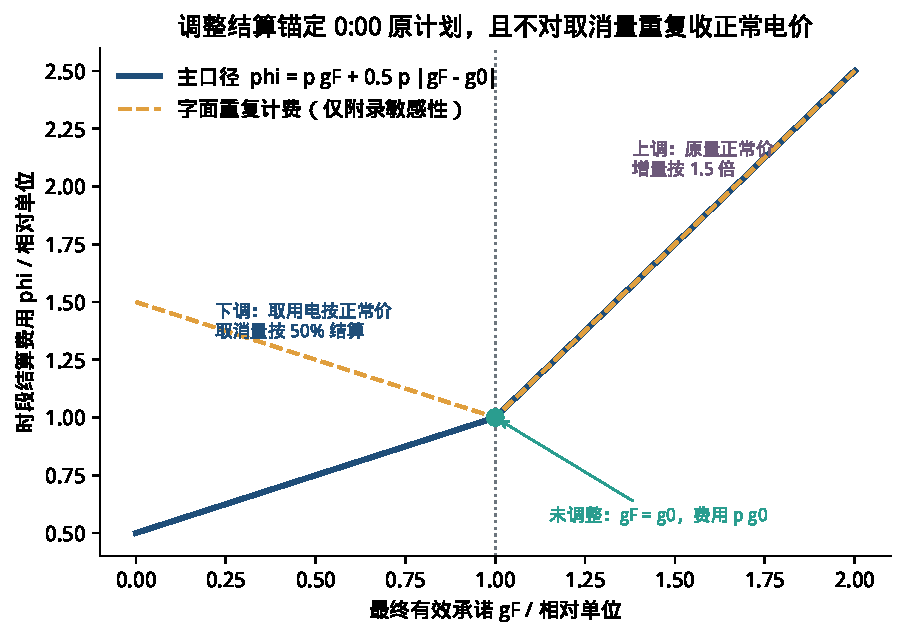
\includegraphics[width=0.72\textwidth]{../fig/q3_paper/fig3_settlement_phi.pdf}
\caption{以 0:00 原计划为锚点的调整结算。实线为主口径~\eqref{eq:q3-phi}；虚线把下调取消量同时按正常价和 50\% 计价，只作附录敏感性，以免把题意歧义写成唯一市场事实。}
\label{fig:q3-phi}
\end{figure}

\subsubsection{主模型：四时点滚动重优化}

物理可行性与问题一、问题二相同。公共母线能量平衡与 SOC 转移为
\begin{equation}
\label{eq:q3-balance}
x_{d,t}+e_{d,t}+P_{d,t}-w_{d,t}+r_{d,t}=L_{d,t}+c_{d,t},
\end{equation}
\begin{equation}
\label{eq:q3-soc}
E_{d,t}=E_{d,t-1}+\eta_c c_{d,t}-\frac{r_{d,t}}{\eta_d}.
\end{equation}
普通购电只能在当期承诺内取用，\(0\le x_{d,t}\le g_{d,t}\)；多余承诺已经按~\eqref{eq:q3-phi} 结算，但不能凭空转移到其他时段。跨时搬运只能经过“购电或光伏 \(\to\) 充电 \(\to\) SOC \(\to\) 放电”。在正电价、无上网收益且电池有损耗时，同时充放电被更低损耗的等价解支配；求解后仍审计 \(c_{d,t}r_{d,t}=0\)。

\paragraph{M0：0:00 后不调整。}
以 0:00 的 \((\widehat L,\widehat P^{0})\) 制订 \(g^{0}\)，此后强制 \(g^{F}=g^{0}\)。它回答“新预测总体上有没有货币价值”：任何允许更新的策略，必须在同一初始 SOC、同一结算和同一执行规则下给出更低的实现成本~\eqref{eq:q3-total-cost}，否则更新权利只是名义上的。

\paragraph{M1：每次更新都评估并求解。}
设更新时刻 \(\tau\) 的当前真实 SOC 为 \(E_{d,\tau}\)，更新前承诺为 \(g^{\mathrm{pre}}\)。在剩余时域 \(\mathcal T_\tau\) 上解
\begin{equation}
\label{eq:q3-m1}
\boxed{
\left\{
\begin{aligned}
\min_{g,x,e,c,r,w,E}\quad
&\sum_{t\in\mathcal T_\tau}
\bigl[\phi_t(g^{0}_{d,t},g_{d,t})+5p_t e_{d,t}\bigr]
+V_{d+1}(E_{d,144}),\\
&g_{d,t}=g^{\mathrm{pre}}_{d,t},\qquad t\notin\mathcal T_\tau,\\
&0\le x_{d,t}\le g_{d,t},\qquad g_{d,t}\ge 0,\\
&\text{以及~\eqref{eq:q3-balance}--\eqref{eq:q3-soc} 与功率、SOC、弃光边界。}
\end{aligned}
\right.}
\end{equation}
规划阶段的平衡使用 \((\widehat L_{d,t},\widehat P^{\tau}_{d,t})\)；执行当前一步时改用真实 \((L_{d,t},P_{d,t})\)，只实施本步动作，下一时段带入真实 SOC 再滚动。这不是预知未来光伏或未来负荷的事后最优。因为 \(g=g^{\mathrm{pre}}\) 始终可行，并且调整价格已经进入目标，模型只有在改计划后仍能降低预计总成本时才会离开原承诺。因而 M1 的“每次更新”是指每次都求解，而不是强迫计划变化。

\paragraph{M6：用信息价值记录是否实施调整。}
在 \(\tau\in\{6{:}00,12{:}00,18{:}00\}\) 计算
\begin{equation}
\label{eq:q3-voi}
\begin{aligned}
J^{\mathrm{fix}}_{\tau}&=\min\{J_{\tau}:g_{d,t}=g^{\mathrm{pre}}_{d,t},\ t\in\mathcal T_\tau\},\\
J^{\mathrm{free}}_{\tau}&=\min\{J_{\tau}:g_{d,t}\ge 0,\ t\in\mathcal T_\tau\},\\
VoI_{\tau}&=J^{\mathrm{fix}}_{\tau}-J^{\mathrm{free}}_{\tau}.
\end{aligned}
\end{equation}
仅当 \(VoI_{\tau}>\varepsilon\) 时写入新承诺，否则维持 \(g^{\mathrm{pre}}\)。\(\varepsilon=0.01\) 元取求解器货币容差，只防止无意义的浮点微调。当保持原承诺可行、调整费进入目标且 \(\varepsilon\to 0\) 时，M1 与 M6 给出同一经济最优解。因此 M6 不是第二个独立主算法，而是 M1 的可解释实施层：它把“新预测值不值得用”写成逐时点的 \(VoI\) 台账。真正有信息含义的比较是
\[
\text{M0},\quad
\text{M1/M6},\quad
M_{6},\ M_{12},\ M_{18},
\]
其中后三个消融各自只开放一个更新时点，用于回答哪一次预报对实现成本最关键。图~\ref{fig:q3-voi} 给出该实施逻辑。

\begin{figure}[H]
\centering
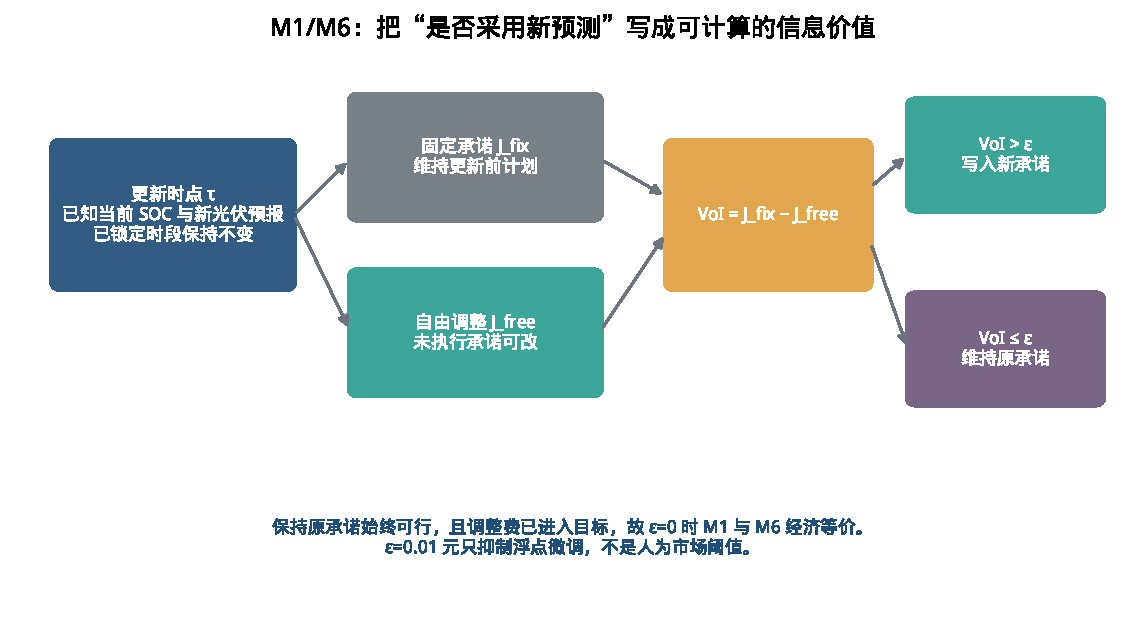
\includegraphics[width=0.92\textwidth]{../fig/q3_paper/fig3_voi_decision.pdf}
\caption{更新时点上的信息价值判定。由于不调整始终可行，\(VoI\) 不会人为制造成本差；单时点消融而不是 M1 对 M6 的成本差，才是“哪个时刻的预测值得使用”的证据。}
\label{fig:q3-voi}
\end{figure}

\paragraph{终端价值。}
日末不强制回到日初 SOC。为避免最后数小时透支电池，优化视域延长到次日，或等价加入到达项 \(V_{d+1}(E_{d,144})\)。该项与问题二政策一致方案相同：由次日基准预测 LP（而非情景全路径补救）在若干 SOC 样本上生成凸支持割，并以弦线--切面间隙作为误差证书。预测输入改用问题三的因果负荷与附件 3 更新口径。它只引导今日末库存，次日购电计划必须到次日 0:00 重新制订，不得提前写入结果文件或重复计费。

\subsubsection{求解算法}

式~\eqref{eq:q3-m1} 在固定预测轨迹下是线性规划：\(\phi_t\) 的绝对值由非负上、下调变量线性化，能量平衡与 SOC 均为线性等式，容量与功率均为盒约束。主求解使用 LP（HiGHS）；若出现数值上的同时充放电，先以最小吞吐量作词典序次目标，仅在仍不能消除时用互斥二元变量复核。选择 LP 而不是遗传算法或完整多阶段随机动态规划，是因为：题目的调整费和紧急电价已经给出可加的货币目标；承诺跨时段的耦合由 SOC 线性传递；计算瓶颈在于全年、多策略、每 10 分钟滚动，而不是非凸组合爆炸。完整情景树（规格中的 M5）能够刻画未发生光伏误差的条件残差，但要求购电承诺跨情景一致、控制动作服从信息历史，不能把每条未来轨迹的储能当作日初指令。M5 只作为不确定性扩展，不替代 M1/M6 的主结果；在其全年审计完成前，正文不把问题三称为严格多阶段随机最优控制。

算法流程如下。对每个策略、每一日：用~\eqref{eq:q3-load} 与 0:00 光伏映射形成日初信息并求解 \(g^{0}\)；在允许的更新点比较 \(J^{\mathrm{fix}}\) 与 \(J^{\mathrm{free}}\)；每个 10 分钟只执行当前动作并更新真实 SOC；日成本按~\eqref{eq:q3-total-cost} 归集。全年比较时，每个策略必须从 2025-01-01 的 6000 kWh 起沿\textbf{自身}决策连续传递 SOC，不得借用 M0 或其他策略的库存路径。1 月用于状态预热与预测历史，题设结果表覆盖 2--12 月；若报告年度成本，须写明是 1--12 月完整核算还是 2--12 月输出区间，二者不得混报。

\subsubsection{结果与机制解释}
\label{sec:q3-results}

本节数字一律待队长把因果负荷主路径写入 \texttt{results\_summary.md} 后再填。当前两日试算使用了当天完整真实负荷，只证明结算公式、锁定窗口和物理残差链路可运行，不能代表现实可执行的日前/日内策略。

待填的主比较应同时给出总成本、普通结算成本、紧急购电成本和弃光，避免把“调整次数多”直接写成“更好”。预期的机制解释（有签收数字后按实际符号改写，不得预先断言全年排序）是：允许更新的策略如果优于 M0，其来源应是\textbf{减少 5 倍紧急补购}，而普通结算成本完全可能上升——因为上调按 1.5 倍付费，模型只有在避免紧急购电的收益超过调整费时才会增加 \(g\)。单时点消融若出现“仅 6:00 更新的实现成本劣于 M0”，原因通常是过早下调后，后续真实光伏/负荷偏差无法在已锁定期内用正常购电挽回，只能转化为紧急购电或被动弃光；这恰恰说明 \(VoI\) 是当时信息下的预测收益，不是实现路径上的保证收益。18:00 更新若增量很小，则因为剩余时段短、可改电量少，且日末库存已由 48 小时到达项约束。

\begin{table}[H]
\centering
\caption{问题三主比较（因果负荷、线性锚点映射、0:00 锚定结算；数字待签收）}
\label{tab:q3-strategy}
\begin{tabular}{lcccc}
\toprule
策略 & 总成本 / 元 & 相对 M0 & 普通结算 / 元 & 紧急成本 / 元 \\
\midrule
M0（不调整） & \QThreeMZeroCost & --- & \QThreeUnsigned & \QThreeUnsigned \\
\(M_{6}\) 仅 6:00 & \QThreeUnsigned & \QThreeUnsigned & \QThreeUnsigned & \QThreeUnsigned \\
\(M_{12}\) 仅 12:00 & \QThreeUnsigned & \QThreeUnsigned & \QThreeUnsigned & \QThreeUnsigned \\
\(M_{18}\) 仅 18:00 & \QThreeUnsigned & \QThreeUnsigned & \QThreeUnsigned & \QThreeUnsigned \\
M1/M6（三点均评估） & \QThreeMainCost & \QThreeSavePct & \QThreeSettleLift & \QThreeEmergDrop \\
\bottomrule
\end{tabular}
\end{table}

指定展示日的计划购电量、调整购电量、四小时充放电与紧急购电按题设 \texttt{result3.xlsx} 列出。正文须同时说明该日 0:00 原计划、各更新点 \(VoI\) 以及调整方向，避免只贴最终 \(g^{F}\)。题设导出区间为 2025-02-01 至 2025-12-31；1 月不写入结果表，但跨日 SOC 必须从年初连续而来。

不得把问题二已签收的 2--12 月成本 14{,}456{,}670.55 元，或政策一致部署路径的 2--12 月成本，与问题三年度成本直接相减。两问结算对象不同（问题二按锁定额度 \(q\) 付费，问题三按 \(\phi(g^{0},g^{F})\) 付费），信息集也不同。对照只能在队长同时签收两问主口径、并统一首末 SOC 与核算区间之后，分项列出计划/调整/紧急三项。

\subsubsection{验证、敏感性与表述边界}

必须通过、且论文只声称“通过数值审计”的项目包括：逐 10 分钟能量平衡与 SOC 递推残差达到数值求解量级；SOC、功率、弃光边界无违例；更新点之前的 \(g\) 不被改写；\(x\le g\)；无同时充放电；\(\phi\) 对上调、下调、未调三类样本与分段定义一致；主模型对当天尚未发生的负荷做扰动时，当时计划不变。\(\texttt{actual\_load\_proxy}\) 必须单独成表，不能并入主比较。

小时预报到 10 分钟的线性锚点映射不是附件唯一规定，分段常数映射只作敏感性。主结算不是题意的唯一读法，相邻版本逐次结算只作附录。在这些全年组合跑完以前，只可以写“两日回归样本未改变审计结论”，不可以写“全年映射与结算解释下策略排序均稳健”。年末 1200 kWh 与 6000 kWh 是核算边界：前者允许释放期初库存，后者要求年末仍保留该库存；成本差应首先解释为库存会计，其次才检查是否改变策略排序。控制器能够即时获得当前负荷/光伏，是本文的控制信息假设，题目未给出通信延迟，故不把结果写成工程部署方案。

图~\ref{fig:q3-overview} 总结问题三在四问主线中的位置：它只放宽承诺改写的时点，不另起一套储能物理。

\begin{figure}[H]
\centering
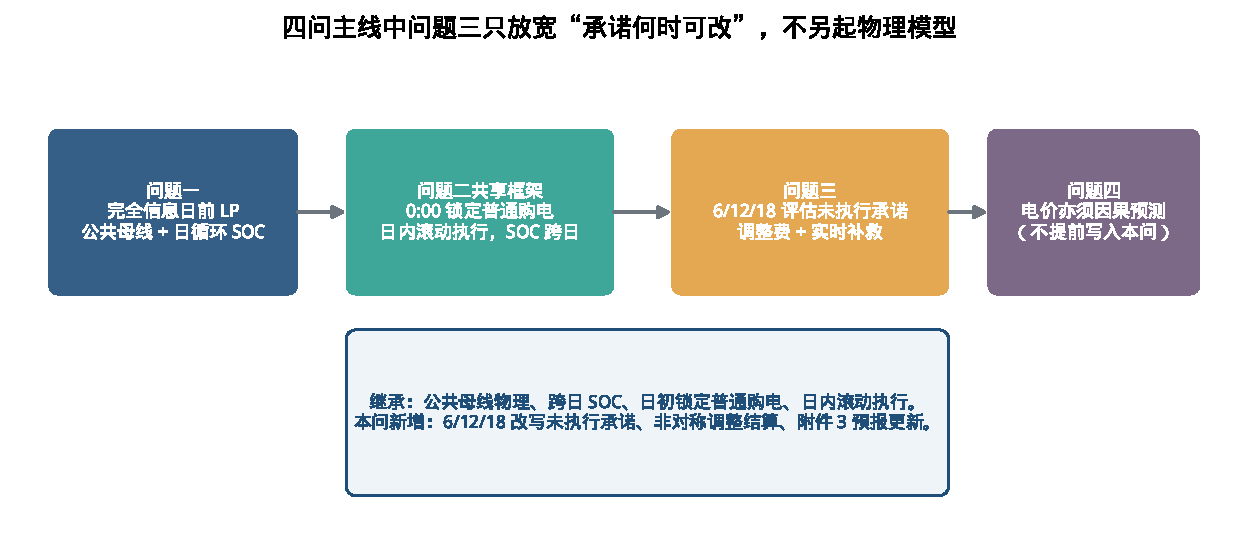
\includegraphics[width=0.96\textwidth]{../fig/q3_paper/fig3_q2_to_q3_overview.pdf}
\caption{问题三在全文主线中的位置。评委从本图应读出：储能物理连续继承，信息集按问递进；本问只放宽普通购电承诺的改写时点，并把调整费计入目标。}
\label{fig:q3-overview}
\end{figure}

% 摘要可用段落（数字仍为宏）
% \textbf{针对问题三，}由于光伏预测在 0:00、6:00、12:00、18:00 更新，若继续全日锁定普通购电，将放弃题目允许的调整权并放大紧急购电。因此以 0:00 原计划为唯一结算锚点，建立计入非对称调整费的剩余时域滚动 LP，并用预测成本差 \(VoI\) 记录是否实施调整。主方案在因果负荷与线性锚点映射下的实现成本为 \QThreeMainCost 元，相对从不调整的 M0 为 \QThreeSavePct。该差额来自紧急购电下降与普通结算变化的对冲，而不是取消调整费或预知未来实际曲线。
